% =====================================================================
%  한글 Term Report (self-contained, 상세본)
%  컴파일: xelatex main.tex  (권장) 2회
% =====================================================================
\documentclass[11pt,a4paper]{article}

\usepackage[a4paper,margin=1in]{geometry}
% 한글: kotex 있으면 사용(Overleaf/full TeX 권장), 없으면 macOS 폰트로 fallback
\IfFileExists{kotex.sty}
  {\usepackage{kotex}}
  {\usepackage{fontspec}\setmainfont{Apple SD Gothic Neo}}
\usepackage{booktabs}
\usepackage{array}
\usepackage{tabularx}
\usepackage{longtable}
\usepackage{amsmath,amssymb}
\usepackage{graphicx}
\usepackage{caption}
\captionsetup{font=small,labelfont=bf}
\usepackage{xcolor}
\usepackage{microtype}
% --- 의존성 없는 pseudocode 프레임 (BasicTeX/Overleaf 모두 컴파일) ---
\usepackage{float}
\makeatletter
\setlength{\@fptop}{0pt}
\makeatother
\newfloat{algorithm}{htbp}{loa}
\floatname{algorithm}{Algorithm}
\newcounter{pcln}
\newenvironment{pcode}{%
  \begin{list}{\scriptsize\arabic{pcln}:}{%
    \usecounter{pcln}\small
    \setlength{\leftmargin}{2.2em}\setlength{\labelwidth}{1.6em}%
    \setlength{\itemsep}{1.5pt}\setlength{\parsep}{0pt}\setlength{\topsep}{3pt}}%
}{\end{list}}
\newcommand{\kw}[1]{\textbf{#1}}                       % 키워드
\newcommand{\ind}{\hspace*{1.3em}}                     % 들여쓰기
\newcommand{\cmt}[1]{\hfill{\footnotesize$\triangleright$\,\textit{#1}}}  % 주석
\emergencystretch=3em
\tolerance=2000
\hbadness=3000
\usepackage{hyperref}
\hypersetup{colorlinks=true, linkcolor=blue!50!black, citecolor=blue!50!black, urlcolor=blue!50!black}

\graphicspath{
  {./figs/}
  {../../exp/v5.2/Plot/loss/}
  {../../exp/v5.2/3_evaluation/10_convergence_similarity/fvt/checkpoint-50000/family_similarity/}
  {../../exp/v5.2/0_tokenizer/03_tokenization_effect/}
}

\newcommand{\rand}{\texttt{random}}
\newcommand{\meanm}{\texttt{mean}}
\newcommand{\fvt}{\texttt{fvt}}
\newcommand{\wfvt}{\texttt{weighted\_fvt}}
\newcommand{\famm}{\texttt{family\_mean}}
\newcommand{\dn}{$\downarrow$}
\newcommand{\up}{$\uparrow$}

\title{XLM-R 기반 저자원 언어 Vocabulary Extension:\\ Family-aware Embedding Initialization과 수렴 분석}
\author{Jongha Kim \\
서강대학교}
\date{Term Project Report (한글본) \\ 2026년 7월}

\begin{document}
\maketitle

% =====================================================================
\begin{abstract}
\noindent
XLM-R은 100개 언어를 학습한 강력한 multilingual masked language model(MLM)이지만, 학습에 포함되지 않은 tail language에서는 한 단어가 여러 subword로 과도하게 쪼개지고(over-fragmentation) 어휘·형태 정보가 표현 공간에 정렬되지 않는 문제가 남는다. Glot500은 mixed corpus로 SentencePiece unigram tokenizer를 재학습해 vocabulary를 확장하고 확장 모델을 MLM으로 continued pretraining하여 이 문제를 완화했으며, 관련 언어가 함께 있을 때 저자원 언어 표현이 좋아지는 related-language help를 보고했다. 본 보고서의 핵심 novelty는 새 token embedding 초기화에 source subtoken 정보와 related-language/family prior를 명시적으로 주입하고, 어떤 prior가 실제 downstream에서 더 안정적인지 통제 비교하는 것이다.

본 보고서는 \fvt\ 의 길이 가중 변형 \wfvt\ 와 family-aware initialization인 \famm\ 을 핵심 변형으로 둔다. 비교를 위해 \rand, \meanm, 표면형 subtoken 재사용 방식인 \fvt\ 도 함께 평가한다. \texttt{xlm-roberta-base} 위에서 92개 XLM-R-seen replay 언어와 7개 XLM-R-unseen target(Target7)을 사용하고, tokenizer는 Glot500 방식으로 고정한 채 초기화만 바꿔 동일한 corpus·objective·schedule·evaluation protocol로 50K-step까지 continued MLM pretraining을 수행한다. 평가는 Glot500 downstream suite(pseudoperplexity, Tatoeba/Bible retrieval, NER, roundtrip alignment, text classification)로 하며, 시작점인 XLM-R-B와 XLM-R-L을 baseline으로 둔다.

세 가지를 관찰한다. (1) 확장 tokenizer는 Target7의 tokens/word를 2.204에서 1.592로 27.75\% 낮춘다. (2) 50K downstream에서는 \wfvt\ 가 PPPL head/all, Tatoeba head/all, Bible 전 group, Roundtrip 전 group에서 최고이고 MLM loss도 가장 낮아 종합적으로 가장 안정적이다. \famm\ 은 tail PPPL·Tatoeba와 NER head/all에서 최고라 family prior가 특정 target 지표에 유효함을 보인다. (3) 2D similarity map의 family clustering은 모델이 유사 family 언어를 가까운 표현 공간에 묶어 학습함을 보여주며, 이는 Glot500의 related-language help와 같은 방향이다. 요컨대 저자원 vocabulary adaptation에서 embedding initialization은 수렴과 downstream 성능을 실제로 바꾸며, 전체 균형에서는 \wfvt, 계통 prior가 필요한 일부 target 지표에서는 \famm\ 이 강하다.
\end{abstract}

% =====================================================================
\section{서론}

\subsection{Vertical scaling과 horizontal scaling}
대규모 언어모델의 발전은 두 축으로 나뉜다. \textbf{Vertical scaling}은 같은 문제를 더 잘 풀기 위해 파라미터 수·학습 데이터 양·모델 깊이·연산량을 키우는 방향으로, ChatGPT·Claude 및 scaling-law 연구가 여기에 속한다. \textbf{Horizontal scaling}은 ``더 많은 대상을 지원할 수 있는가''를 묻는 방향으로, 더 많은 언어·도메인·태스크를 포괄한다. 데이터가 적은 저자원 언어 지원은 전형적인 horizontal scaling 문제이며 본 보고서의 배경이다. XLM-R은 강력한 multilingual encoder지만 학습에 없던 언어에서는 (1) token fragmentation, (2) representation mismatch가 남는다.

\subsection{선행 해법과 남은 빈틈}
Glot500은 horizontal scaling을 위해 vocabulary extension과 continued MLM pretraining을 결합한다(자세한 파이프라인은 \S2). 그러나 vocabulary extension 이후 새 token embedding row의 \emph{초기값}은 여전히 열린 선택이다. XLM-R의 embedding matrix는 250{,}002개 token에 대한 행렬 $E\in\mathbb{R}^{250002\times768}$이다. tokenizer를 확장해 116{,}664개 새 piece를 붙이면 $E$는 $\mathbb{R}^{366666\times768}$로 커지는데, 새로 늘어난 116{,}664개 행은 사전학습에서 한 번도 gradient를 받은 적이 없는 ``빈 행''이다. continued pretraining은 이 빈 행들을 학습으로 채우지만, \emph{어디서 출발하느냐}가 최적화 궤적과 최종 표현을 바꿀 수 있다.

기존 연구가 주로 쓰는 방법은 세 가지다. \rand\ 는 아무 정보 없이 무작위 벡터에서 시작하고, \meanm\ 은 기존 embedding들의 전역 평균(중심)에서 안정적으로 시작하며, \fvt\ 는 새 token의 표면형을 기존 tokenizer로 다시 쪼개 그 구성 subtoken embedding의 평균을 재사용한다. 즉 정보량은 무정보 \rand, 전역 centroid \meanm, 표면형 재사용 \fvt\ 순으로 늘어난다. 본 보고서는 여기에 두 방법을 추가한다. \wfvt\ 는 FVT의 subtoken 평균을 균등 평균 대신 \emph{표면 길이로 가중}한다 --- 긴 source subtoken일수록 더 구체적인 lexical 신호를 담는다는 가정이다. \famm\ 은 표면형 분해가 아니라, 새 token이 corpus에서 주로 유래한 언어의 \emph{language family}에 속한 source token들의 평균을 쓴다 --- 철자보다 계통(typology) prior가 저자원 token에 더 좋은 출발점을 주는지 확인하기 위함이다. 이로써 비교 축이 다섯 방법으로 확장된다.

\subsection{기여}
\begin{enumerate}\setlength\itemsep{0.15em}
\item Source subtoken 정보를 길이 가중으로 재사용하는 \wfvt\ 와 Glot500의 related-language help를 새 token row 초기화로 옮긴 family-aware \famm\ 을 제시하고, tokenizer를 고정한 5-way ablation으로 검증한다.
\item 2D similarity map의 family clustering과 downstream task 결과를 연결해, \wfvt\ 가 가장 강한 종합 초기화이고 계통 기반 \famm\ 은 tail PPPL·Tatoeba와 NER head/all에서 강한 값을 보임을 보인다.
\item 문장 표현 공간의 계통 구조가 학습 과정에서 어떻게 형성되는지 step별로 분석하고, 이를 초기화 prior 선택의 해석 근거로 사용한다.
\end{enumerate}

% =====================================================================
\section{관련 연구 (Previous Research)}

\subsection{Glot500과 horizontal language scaling}
Glot500은 high-resource 언어의 기존 표현 지식을 기반으로 언어 간 전이를 확장하는 horizontal scaling 접근이다. 종교 텍스트(성경·종교 번역문), 뉴스 기사, 과학 논문, 위키/웹 크롤링 등 다양한 도메인의 데이터를 모아 저자원 언어를 포함한 대규모 corpus(Glot500-c)를 구축한다.

\paragraph{Corpus collection.} 저자원 언어는 고품질 데이터셋 확보가 어려워 web crawling으로 원천을 모은 뒤 data cleaning을 거친다. (1) \textbf{Language-Scripts}: 언어만이 아니라 language-script 단위(예: 같은 언어라도 다른 문자)로 분리해 tokenization 병목을 구분한다. (2) \textbf{N-gram LM과 language divergence}: 각 language-script corpus에 대해 3-gram 언어모델을 만들고 perplexity를 비교하여 잘못 라벨링된 corpus를 걸러낸다. (3) \textbf{Chunk-level filter}: 반복 문자·반복 단어·특수문자·너무 짧은 텍스트·중복 데이터를 제거한다. (4) \textbf{Corpus-level filter}로 최종 정제한다. 마지막으로 학습 단위(chunk)가 30{,}000개 이상인 language-script만 선별한다. 여기서 학습 단위(논문 표기 ``sentence''')는 완전한 한 문장일 수도, 짧은 구절일 수도, 여러 문장이 묶인 paragraph일 수도 있다 --- 언어마다 텍스트 특성이 달라 수집된 단위를 그대로 처리하기 위한 묶음이다.

\paragraph{Tokenization.} subword tokenizer로는 자주 함께 등장하는 문자 쌍을 반복적으로 병합하는 \textbf{BPE}와, 처음에 많은 subword 후보를 두고 문장을 가장 잘 설명하는 조합만 남기는 \textbf{Unigram Language Model}이 있다. Glot500은 SentencePiece의 Unigram LM을 쓴다. 미등록 조각 처리로는 미등록 subword를 Unicode 문자 단위로 분해하는 \emph{character fallback}(unknown token 발생 가능)과, 미등록 문자를 UTF-8 byte 단위로 분해하는 \emph{byte fallback}이 있으며, 후자는 unknown을 만들지 않는다. multilingual model에서 tokenizer 품질과 fertility가 실제 성능에 영향을 준다는 점은 Rust et al.\ 이 체계적으로 보였고, XLM-R/mBERT에 없는 script를 다룰 때는 unknown·fragmentation 문제가 더 직접적으로 나타난다\cite{rusttok,pfeifferunks}. CANINE 같은 tokenization-free encoder는 이 병목을 아예 제거하는 대안이지만\cite{canine}, 본 보고서는 XLM-R/Glot500 계열과 비교 가능성을 유지하기 위해 subword vocabulary extension 축에 집중한다.

\paragraph{MLM continued pretraining.} Glot500-m은 약 600GB corpus 위에서 두 단계로 만들어진다. (1) \emph{Vocabulary Extension}: 기존 XLM-R tokenizer vocabulary를 확장한다(원 논문은 새 행을 random으로 초기화). (2) \emph{Continued Pretraining}: XLM-R-base를 Glot500-c로 이어서 MLM 학습한다. 이때 언어별 데이터 양 편차가 크므로 temperature $\alpha=0.3$의 언어 sampling을 적용해 head 언어가 학습을 독점하지 않도록 한다(본 실험도 동일 $\alpha$를 쓴다, \S3.3).

\paragraph{Glot500의 분석.} Glot500은 성능이 corpus 크기, script coverage, 관련 언어 지원, 모델 용량이 함께 작용해 결정된다고 본다. 특히 주변의 유사(계통) 언어가 함께 학습될 때 표현이 좋아지며(related-language help), 반대로 가까운 관련 언어가 없으면 특정 언어 하나만 이어 학습한 Glot+1이 511개를 함께 학습한 Glot500-m보다 나은 경우도 있다. 본 보고서의 \famm\ 초기화와 계통 구조 분석(\S6)은 이 관찰과 직접 연결된다.

\subsection{Vocabulary extension의 두 계열}
Glot500 계열은 seen 언어와 unseen 언어를 함께 담은 mixed corpus로 새 SentencePiece unigram tokenizer를 학습해 vocabulary를 확장한다. 반면 Yamaguchi et al.\ 의 저자원 vocabulary expansion은 아주 적은 target language text(약 0.01GB)만으로 auxiliary tokenizer를 새로 학습한 뒤, 기존 source vocab에 없는 target token만 골라 뒤에 append하고 짧게 이어 학습한다. 최근 연구들도 vocabulary expansion을 단순 전처리가 아니라 append 규모, 학습 budget, embedding initialization이 결합된 adaptation 문제로 다룬다\cite{yamaguchi,mundra2024,lin2025}. 두 방식은 새 vocab을 정하는 데이터(대규모 mixed corpus인지 소량 target-only인지)와 붙이는 token 수에서 다르다. 본 보고서는 \textbf{main axis를 Glot500식 mixed-corpus vocab injection으로 고정}하고 초기화만 비교하며, Yamaguchi식은 별도 추가 실험 대상으로 남긴다. 요점은, ``vocabulary를 확장한다''는 것이 하나의 고정된 절차가 아니라 tokenizer 학습 데이터·append 정책·초기화의 여러 선택으로 이루어진다는 것이며, 본 보고서는 그중 \emph{초기화}에 집중한다.

\subsection{Embedding initialization / vocabulary transfer}
새 vocabulary 행을 기존 embedding 공간에 잘 배치하는 문제는 cross-lingual vocabulary transfer에서 다뤄져 왔다. Artetxe et al.\ 은 transformer body를 고정하고 새 embedding matrix만 학습해도 cross-lingual transfer가 가능함을 보여, lexical/embedding layer가 새 언어 adaptation의 핵심 bottleneck임을 보였다\cite{artetxe2020}. 이후 mini-model adaptation은 새 embedding 학습 비용을 줄이는 방향으로 이 계열을 확장했다\cite{marchisio2023}. \textbf{FVT}(Fast Vocabulary Transfer)는 새 token 표면형을 source tokenizer로 재분해해 구성 subtoken embedding 평균을 쓰며, 본 실험의 \fvt\ 가 이 방법을 그대로 구현한 것이다(main hypothesis).

본 보고서가 \textbf{WECHSEL}과 \textbf{FOCUS}를 함께 소개하는 이유는, 이들이 ``새 token의 초기값을 무작위로 두지 말고 기존 embedding 공간의 유사한 방향에서 시작하라''는 본 실험의 문제의식을 뒷받침하는 대표적 선행연구이기 때문이다. WECHSEL은 정적 다국어 word embedding에서 new token과 source token 사이의 유사도를 계산해, 유사한 source token들의 가중 평균으로 새 행을 초기화한다. FOCUS는 source vocab과 겹치는 anchor token의 임베딩을 기준으로 new token을 그 조합으로 표현한다. 두 방법 모두 ``의미·표면 유사성을 재사용하면 무작위보다 좋은 출발점을 얻는다''는 것을 보였고, 이는 우리가 계통 유사성을 재사용하는 \famm\ 을 제안한 직접적 동기가 된다. Mundra et al.\ 은 여러 initialization을 RoBERTa/LLaMA2 확장 조건에서 비교해 convex-hull/단순 초기화도 강한 baseline이 될 수 있음을 보였고, Sakajo et al.\ 은 bilingual dictionary만으로도 low-resource vocabulary transfer를 구성할 수 있음을 보인다\cite{mundra2024,sakajo2025}. 다만 WECHSEL/FOCUS/사전 기반 방법은 외부 정적 임베딩, anchor 계산, 또는 bilingual dictionary를 요구해 파이프라인이 무거우므로, 본 실험에서는 구현하지 않고 배경으로만 인용한다. \textbf{Hewitt}류는 새 embedding을 기존 분포의 평균 근처에 두면 초기 불안정을 줄일 수 있다는 근거로, \meanm\ baseline의 배경이다.

\subsection{평가 프로토콜}
Glot500 downstream suite와 pseudoperplexity를 따른다(본 보고서는 retrieval·NER·roundtrip·text classification과 PPPL을 보고). Glot500은 저자원 언어에 labeled train set이 없음을 명시하고 supervised task를 \emph{English로 fine-tune한 뒤 target zero-shot 전이}(XTREME 방식)로 평가한다. 원문: ``Since training data does not exist for some languages, we finetune on English (with early stopping based on dev) and evaluate zero-shot transfer.'' 이 설정을 쓰는 이유는 명확하다 --- target 언어에 labeled 데이터가 없어 target fine-tune이 불가능하고, English로만 supervision을 주면 target 성능이 나오는 유일한 경로가 \emph{공유 multilingual 표현의 cross-lingual 정렬}뿐이라, 이 정렬이 곧 vocabulary extension·initialization이 바꾸는 대상이기 때문이다. 각 task의 구체적 동작·코드는 \S5에 정리한다.

% =====================================================================
\section{데이터}

\subsection{언어 범위와 데이터 출처}
Corpus universe는 99개 language-script로, 92개 head/replay 언어와 7개 target(Target7)로 나뉜다. 두 그룹의 포함 관계는 다음과 같다.
\begin{itemize}\setlength\itemsep{0.1em}
\item \textbf{head 92개}: XLM-R 학습에 \emph{포함된} 언어에서 골랐다(XLM-R이 이미 표현을 가진 high-resource replay 집합). continued pretraining 동안 이들을 함께 학습해 기존 표현을 잊지 않도록(catastrophic forgetting 방지) 유지한다.
\item \textbf{target 7개(Target7)}: XLM-R 학습에 \emph{포함되지 않은}(unseen) 언어다. 다만 Glot500-c에는 존재하므로, 우리는 이들의 원천 텍스트를 Glot500 raw corpus에서 가져온다.
\end{itemize}
즉 두 그룹 모두 학습 텍스트의 출처는 \textbf{Glot500-c}이며, 언어당 HuggingFace Arrow 데이터셋(\texttt{\{lang\}\_\{script\}}, \texttt{train} split의 \texttt{text} 컬럼)으로 관리한다(전처리: \path{preprocessing/merge_files.py}). Target7은 (i) XLM-R-unseen, (ii) Glot500 corpus 존재, (iii) \texttt{new\_length}$\ge$30{,}000, (iv) downstream 평가 데이터 확보 가능이라는 네 조건으로 선별했다. 평가 데이터의 출처는 각각 공개 벤치마크다: retrieval은 Tatoeba와 Parallel Bible Corpus(PBC), NER은 WikiANN, text classification은 Taxi1500이다(\S5).

\begin{table}[H]\centering\small
\caption{Target7 언어와 각 언어가 커버하는 평가 task.}
\begin{tabular}{@{}llllr>{\raggedright\arraybackslash}p{3.6cm}@{}}
\toprule
language\_script & full name & family & region & new\_length & Covered tasks \\
\midrule
\texttt{dtp\_Latn} & Kadazan Dusun & Austronesian & SE Asia & 48{,}468 & Tatoeba, Bible, Roundtrip, Taxi, Embedding \\
\texttt{xav\_Latn} & Xavante & Macro-Je & S America & 31{,}765 & Bible, Roundtrip, Taxi \\
\texttt{bam\_Latn} & Bambara & Mande & W Africa & 32{,}150 & Bible, Roundtrip, Taxi \\
\texttt{csb\_Latn} & Kashubian & Slavic & Europe & 33{,}743 & Tatoeba, NER, Embedding \\
\texttt{ile\_Latn} & Interlingue & Constructed & Europe & 40{,}984 & Tatoeba, Embedding \\
\texttt{lij\_Latn} & Ligurian & Romance & Europe & 42{,}447 & NER \\
\texttt{fur\_Latn} & Friulian & Romance & Europe & 30{,}052 & NER \\
\bottomrule
\end{tabular}
\end{table}

\subsection{언어 선택 이유: task 중심 설계}
언어 선택은 임의가 아니라 ``평가까지 연결 가능한 tail language''라는 기준을 따른다. 대부분의 진짜 저자원 언어는 human-labeled downstream 데이터가 전혀 없어 tokenizer$\to$training$\to$evaluation을 끝까지 연결할 수 없다. 그래서 각 downstream task마다 \emph{평가 가능한 target 언어를 최소 3개씩} 확보하도록 7개를 역으로 골랐다. 표~\ref{tab:taskcov}는 이 task 중심 매핑을 보여준다(피드백 반영). 지역·계통도 SE Asia/S America/W Africa/Europe로 분산했다. 이 선택은 일반성보다 traceability를 우선한 결과다.

\begin{table}[H]\centering\small
\caption{Task별 평가 대상 target 언어(각 3개)와 평가 규모.}
\label{tab:taskcov}
\begin{tabular}{@{}lll@{}}
\toprule
Task & target 언어 (3개) & 평가 규모 \\
\midrule
Tatoeba retrieval & \texttt{dtp}, \texttt{ile}, \texttt{csb} & 2{,}253 문장쌍 \\
Bible retrieval & \texttt{dtp}, \texttt{xav}, \texttt{bam} & 23{,}238 문장쌍 \\
Roundtrip alignment & \texttt{dtp}, \texttt{xav}, \texttt{bam} & 22{,}669 문장군 \\
NER & \texttt{csb}, \texttt{lij}, \texttt{fur} & 300 문장 (100/lang) \\
Embedding similarity & \texttt{csb}, \texttt{dtp}, \texttt{ile} & 2{,}100 문장쌍 \\
\bottomrule
\end{tabular}

\vspace{2pt}
{\footnotesize 단위 설명: retrieval의 ``문장쌍''은 English와 target 언어의 병렬 문장(Bible은 같은 verse) 쌍이다. roundtrip의 ``문장군''은 여러 언어를 순환하며 정렬하는 한 세트의 다국어 문장이다. NER은 target 언어 문장 단위(언어당 100)다.}
\end{table}

\subsection{학습 corpus와 sampling}
MLM 학습 corpus는 seen replay와 target을 섞어 구성한다. 표~\ref{tab:corpus}는 실제 개수다.

\begin{table}[H]\centering\small
\caption{학습/평가 데이터 규모(samples).}
\label{tab:corpus}
\begin{tabular}{@{}lr@{}}
\toprule
항목 & 개수 \\
\midrule
source raw sentences & 1{,}025{,}895{,}043 \\
MLM train --- seen/head & 4{,}147{,}176 \\
MLM train --- target7 & 335{,}083 \\
MLM train --- total & 4{,}482{,}259 \\
\midrule
평가 --- PPPL & 700 \\
평가 --- Tatoeba & 2{,}253 \\
평가 --- Bible & 23{,}238 \\
평가 --- Roundtrip & 22{,}669 \\
평가 --- NER & 300 \\
\bottomrule
\end{tabular}
\end{table}

\paragraph{Temperature sampling ($\alpha=0.3$).} vocab size는 고정인데 head 언어를 그대로 많이 넣으면 subtoken이 high-resource 언어에 편향된다. 이를 막기 위해 각 language-script의 샘플링 확률을 데이터 양 $n_i$에 대해
\[
P_i \propto n_i^{\alpha},\qquad \alpha=0.3
\]
로 둔다. 예를 들어 head 1{,}000{,}000 문장과 tail 1{,}000 문장이 있으면, $\alpha=1$에서는 비율이 $1000{:}1$이지만 $\alpha=0.3$에서는 $10^{6\cdot0.3}{:}10^{3\cdot0.3}\approx 8{:}1$로 완화된다. 이 down-weighting은 tokenizer 학습뿐 아니라 \emph{실제 MLM 학습 corpus 생성에도 적용}되어, head 독점과 target overfitting을 동시에 피한다.

% =====================================================================
\section{방법 (Method)}

\subsection{Tokenizer extension}
tokenizer는 Glot500식 \emph{append-only injection}으로 고정한다. 절차는 다음과 같다.
\begin{enumerate}\setlength\itemsep{0.1em}
\item XLM-R의 \texttt{sentencepiece.bpe.model}(250{,}002 vocab)을 source로 복사한다.
\item 99개 language-script mixed corpus($\alpha=0.3$ sampling)에서 SentencePiece \emph{unigram} auxiliary model을 학습한다(\texttt{byte\_fallback=true}, \texttt{character\_coverage=1.0}).
\item source SPM에 \emph{없는} piece만 골라 기존 vocab \emph{뒤에} append한다. HuggingFace \texttt{add\_tokens()}가 아니라 SPM protobuf에 직접 붙여 unigram score를 보존한다.
\end{enumerate}
결과 vocab은 $250{,}002 \to 366{,}666$(신규 116{,}664)이다. 기존 token id는 보존되지만 \verb|<mask>| 같은 special token id는 이동할 수 있어(250001$\to$366665) 초기화 단계에서 string identity로 remap한다(\S4.3).

\paragraph{Yamaguchi 방식과의 차이.} Yamaguchi식은 소량 target-only text로 auxiliary tokenizer를 학습해 필요한 target token만 붙이는 반면, 본 보고서(Glot500식)는 92개 seen과 7개 target을 합친 mixed corpus로 tokenizer를 학습해 훨씬 많은 piece(116{,}664)를 붙인다. 즉 확장 방법 자체가 (tokenizer 학습 데이터·append 규모에서) 여러 갈래인데, 본 실험은 이 축을 고정하고 초기화만 비교한다.

\subsection{Embedding initialization: 다섯 방법}
공통 규칙은 세 가지다. (i) source tokenizer에 이미 있는 token은 source row를 그대로 복사한다. (ii) 새로 추가된 116{,}664개 행만 method별로 초기화한다. (iii) \verb|<mask>| 는 id가 이동하므로 string identity로 remap하고, input embedding과 LM head의 weight tying을 유지한다. 감사 수치: source len 250{,}002 · target len 366{,}666 · new rows 116{,}664 · \verb|<mask>| copy diff 0.0 · LM head tied. 다섯 방법의 핵심 로직은 아래와 같다(근거: \path{scripts/build_v5_initialized_checkpoint.py}).

\begin{algorithm}[h]
\caption{새 vocabulary 행 초기화 (5-way)}
\begin{pcode}
\item \kw{입력:} source embedding $E_{\text{src}}\in\mathbb{R}^{250002\times768}$, 새 token 집합 $T_{\text{new}}$ ($116{,}664$개), method $m$
\item $E \gets [\,E_{\text{src}}\,;\ \mathbf{0}_{116664\times768}\,]$ \cmt{기존 행 복사, 새 행 추가}
\item \kw{for each} 새 token $t$ (id $j$) \kw{do}
\item \ind \kw{if} $m{=}\texttt{random}$: $\ E_j \sim \mathcal{N}(0,\,0.02)$ \cmt{(1) 무정보}
\item \ind \kw{elif} $m{=}\texttt{mean}$: $\ E_j \gets \mathrm{mean}(E_{\text{src}})$ \cmt{(2) 전역 centroid}
\item \ind \kw{elif} $m{=}\texttt{fvt}$: $\ S \gets \mathrm{SrcTok}(\mathrm{surf}(t));\ E_j \gets \mathrm{mean}(E_{\text{src}}[S])$ \cmt{(3) 표면형}
\item \ind \kw{elif} $m{=}\texttt{weighted\_fvt}$: $\ w_s \gets |\mathrm{piece}(s)|;\ E_j \gets \big(\textstyle\sum_{s} w_s E_{\text{src}}[s]\big)/\textstyle\sum_{s} w_s$ \cmt{(4) 길이 가중}
\item \ind \kw{elif} $m{=}\texttt{family\_mean}$: $\ f \gets \mathrm{family}(\mathrm{prov}(t));\ E_j \gets \mathrm{mean}(E_{\text{src}}[\mathrm{SrcTok}(f)])$ \cmt{(5) 계통}
\item $\texttt{<mask>}$ string identity remap ($250001{\to}366665$); \ LM head $\gets$ tie($E$)
\item \kw{return} $E$
\end{pcode}
\end{algorithm}

\paragraph{각 방법의 직관.}
\rand\ 는 $\mathcal{N}(0,0.02)$에서 뽑아 의미 정보 없이 무작위 시작점에서 학습한다. \meanm\ 은 기존 lexical embedding의 평균, 즉 pretrained embedding 공간의 ``중앙값'' 근처에서 안정적으로 시작하되 표면형 정보는 쓰지 않는다. \fvt\ 는 새 token을 기존 tokenizer로 분해한 뒤 그 source subtoken embedding 평균을 써서 표면형/부분형 정보를 살린다(예: 새 token \texttt{\_bambara}가 source에서 \texttt{[\_bam][bara]}로 쪼개지면 두 embedding의 평균에서 출발). \wfvt\ 는 이 평균에 표면 길이 가중을 주어 더 긴(구체적) subtoken을 더 반영한다.

\paragraph{Provenance와 family 분류(\famm).} \famm\ 은 표면형 대신 계통 prior를 쓴다. tokenizer 학습 corpus에서 각 새 token이 \emph{어느 language-script 문장에서 주로 등장했는지}(provenance)를 집계하고, 그 language-script를 언어 메타데이터(\path{miscellaneous/languages_stats.csv}의 \texttt{family} 컬럼)로 language family에 매핑한 뒤, 그 family에 속한 head source 언어들의 token embedding 평균을 새 행의 초기값으로 쓴다. 표~\ref{tab:fam}은 Target7이 실제로 어떤 family로 묶이고 어떤 head 언어를 재사용하는지를 보여준다.

\begin{table}[H]\centering\small
\caption{Target7의 family 분류와 \famm\ 이 참조하는 head source 언어.}
\label{tab:fam}
\begin{tabular}{@{}lll@{}}
\toprule
target & family & 같은 family의 head source 언어 \\
\midrule
\texttt{dtp} & Austronesian & \texttt{ind, msa, jav, tgl, mlg} \\
\texttt{csb} & Slavic & \texttt{ces, hrv, pol, slk, slv} \\
\texttt{fur} & Romance & \texttt{cat, fra, ita, por, ron} (그리고 \texttt{lij}) \\
\texttt{lij} & Romance & \texttt{cat, fra, ita, por, ron} (그리고 \texttt{fur}) \\
\texttt{ile} & Constructed & \texttt{epo} \\
\texttt{bam} & Mande & head에 동일 family 없음(대체: macro-family Niger-Congo의 \texttt{xho}) \\
\texttt{xav} & Macro-Je & head에 동일·근접 family 없음 \\
\bottomrule
\end{tabular}
\end{table}

예컨대 \texttt{dtp}(Austronesian) 유래 token은 \texttt{ind/msa/jav/tgl} 등 Austronesian source token의 평균에서 출발한다. 반대로 \texttt{bam}(Mande)와 \texttt{xav}(Macro-Je)는 head에 같은 계통 언어가 없어 계통 prior의 이점이 제한되는데, 이 대조는 결과 해석(\S6--7)과 직접 연결된다. 같은 family 판정 기준은 표현 공간 분석(\S7)에서도 동일하게 쓴다.

\subsection{Continued MLM pretraining}
확장·초기화된 모델을 \S3.3 corpus 위에서 MLM으로 이어 학습한다. 설정은 표~\ref{tab:mlm}이며, 다섯 방법 모두 동일 exposure로 50K-step까지 학습하고 50K checkpoint 기준으로 보고한다.

\begin{table}[h]\centering\small
\caption{Continued MLM pretraining 설정.}
\label{tab:mlm}
\begin{tabular}{@{}ll@{}}
\toprule
Item & Value \\
\midrule
base model & \texttt{xlm-roberta-base} \\
objective & MLM (dynamic masking, mask prob 0.15) \\
learning rate & $5\mathrm{e}{-}5$ \\
Adam & betas $(0.9,0.999)$, $\varepsilon=1\mathrm{e}{-}8$ \\
LR schedule / warmup / weight decay & linear / 0 / 0.0 \\
max sequence length & 512 \\
language sampling & $\alpha=0.3$ \\
checkpoint interval & 1{,}000 steps \\
convergence budget & 50{,}000 steps (5-way) \\
\bottomrule
\end{tabular}
\end{table}

% =====================================================================
\section{실험: 평가 task와 동작}

다섯 방법은 \emph{초기화만} 다르고 tokenizer·corpus·objective·budget·evaluation runner는 모두 같다. 따라서 점수 차이는 초기화와 그로 인한 training dynamics의 상호작용으로 해석한다. 여기서는 각 downstream task를 왜(선행연구), 어떻게(입력$\to$처리$\to$출력), 그리고 코드 수준으로 정리한다.

\paragraph{공통: 문장 임베딩 추출.} retrieval·similarity는 Glot500 retrieval 방식을 그대로 차용한다.
\begin{algorithm}[h]
\caption{문장 임베딩 추출 (Glot500 retrieval 방식)}
\begin{pcode}
\item \kw{입력:} 문장 $x$, 모델 $M$
\item $H \gets M(x)$ \cmt{hidden states 전체}
\item $h \gets H[\text{layer } 7]$ \cmt{0-index 8번째 layer}
\item $\text{sent} \gets \text{mean-pool}(h,\ \text{mask}=\text{token}\notin\{\text{CLS},\text{SEP},\text{PAD}\})$
\item $\text{sent} \gets \text{L2-normalize}(\text{sent})$ \cmt{similarity 분석 시 전역 평균 차감}
\item \kw{return} $\text{sent}$
\end{pcode}
\end{algorithm}

\subsection{Pseudoperplexity (PPPL) --- \dn}
\textbf{왜.} fine-tuning 없이 모델이 해당 언어 문장을 얼마나 자연스럽게 예측하는지 재는 intrinsic 지표(Salazar et al.\ 2020: PPPL이 좌$\to$우 perplexity보다 언어 acceptability를 잘 반영).
\textbf{입력.} target7 문장 pool. \textbf{처리/출력.} 각 위치를 하나씩 mask하고 정답 token NLL을 합산·지수화. \textbf{해석.} 낮을수록 좋다.
\begin{algorithm}[h]
\caption{Pseudoperplexity (PPPL)}
\begin{pcode}
\item \kw{입력:} 문장 token $\text{ids}$, 모델 $M$; \ $\text{nll} \gets 0$
\item \kw{for} $t = 1$ \kw{to} $|\text{ids}|-2$ \kw{do} \cmt{각 위치를 하나씩 mask}
\item \ind $\text{masked} \gets \text{ids}$, \ $\text{masked}[t] \gets \texttt{<mask>}$
\item \ind $\text{nll} \mathrel{+}= -\log\mathrm{softmax}(M(\text{masked})[t])[\,\text{ids}[t]\,]$ \cmt{정답 token NLL}
\item \kw{return} $\exp(\text{nll} / n_{\text{tokens}})$ \cmt{낮을수록 좋음}
\end{pcode}
\end{algorithm}

\subsection{Sentence Retrieval --- Tatoeba / Bible --- \up}
\textbf{왜.} 두 언어의 같은 의미 문장이 임베딩 공간에서 가까운지, 즉 cross-lingual semantic alignment의 대리 지표(Hu et al.\ 2020, Artetxe \& Schwenk 2019).
\textbf{입력.} English$\leftrightarrow$target 병렬 문장(Tatoeba, 또는 PBC verse-aligned Bible). \textbf{처리.} 양쪽을 임베딩해 각 English 문장의 cosine 최근접 10개를 검색. \textbf{출력.} 정답 짝이 Top-10 안에 들면 hit, 비율이 Acc10.
\begin{algorithm}[h]
\caption{Sentence Retrieval (Top-10 accuracy)}
\begin{pcode}
\item \kw{입력:} target 문장 $\{x_i\}$, English 병렬 문장 $\{y_i\}$ ($i$-th 끼리 정답 쌍)
\item $X \gets \text{L2}(\text{embed}(x))$; \ $Y \gets \text{L2}(\text{embed}(y))$ \cmt{layer-7 mean-pool}
\item \kw{for each} English $y_i$ \kw{do:} \ $\mathrm{top10}(i) \gets$ cosine 최근접 10개 among $\{X\}$
\item \kw{return} $\mathrm{Acc10} = \frac{1}{N}\sum_i \mathbb{1}[\,i \in \mathrm{top10}(i)\,]$
\end{pcode}
\end{algorithm}
Bible은 후보 pool이 언어당 $\sim$7--8천 절로 커 매우 어렵다(\S6.4, Appendix~A).

\subsection{NER --- \up}
\textbf{왜.} English에서 배운 개체명 경계·유형이 다른 언어로 전이되는지(XTREME 표준, WikiANN 데이터). \textbf{처리.} 인코더 위에 token classification head를 얹어 English로 fine-tune 후 target zero-shot. \textbf{출력.} seqeval entity-level F1.
\begin{algorithm}[h]
\caption{NER (English fine-tune, target zero-shot)}
\begin{pcode}
\item \kw{입력:} checkpoint $\theta$, English WikiANN, target 문장
\item token classification head를 $\theta$ 위에 부착
\item \kw{fine-tune} on English: $10$ epoch, LR $2\mathrm{e}{-}5$, batch $8{\times}4$, max\_len $256$
\item $\text{preds} \gets \arg\max$ head(target 문장) \cmt{zero-shot, 학습 없음}
\item \kw{return} $\mathrm{F1} = \mathrm{seqeval}(\text{gold},\ \text{preds})$ \cmt{entity-level, B-/I- 경계}
\end{pcode}
\end{algorithm}
라벨은 BIO 체계의 \texttt{O, B-PER, I-PER, B-ORG, I-ORG, B-LOC, I-LOC}(7개)다. 예: ``Barack$_{\text{B-PER}}$ Obama$_{\text{I-PER}}$ visited$_{\text{O}}$ Paris$_{\text{B-LOC}}$''.

\subsection{Roundtrip Alignment --- \up}
\textbf{왜.} gold 없이 표현 품질을 보는 지표(Dufter et al.\ 2018): 여러 언어를 거쳐 단어 alignment를 돌렸을 때 원래 단어로 돌아오는 비율. \textbf{처리.} 인코더 임베딩으로 인접 언어쌍 word alignment(simalign)를 구하고 cycle을 따라간다. \textbf{출력.} round-trip 복귀율.
\begin{algorithm}[h]
\caption{Roundtrip Alignment (simalign)}
\begin{pcode}
\item \kw{입력:} checkpoint $\theta$, 언어 cycle (예: src$\to$eng$\to$pivot$\to$src)
\item 인접 언어쌍마다 임베딩 기반 word alignment(argmax) 계산
\item \kw{for each} source word $w$ \kw{do:} \ $w' \gets w$ 를 cycle 따라 추적; \ $\text{correct}\mathrel{+}=\mathbb{1}[w'{=}w]$ \cmt{복귀?}
\item \kw{return} $\text{correct} / n_{\text{words}}$
\end{pcode}
\end{algorithm}

\subsection{Text Classification --- Taxi1500 --- \up}
\textbf{왜.} 영어로 fine-tuning한 분류기가 다른 언어에 zero-shot으로 전이되는지(Ma et al.\ 2023). \textbf{처리.} sequence classification head를 English로 fine-tune 후 평가. \textbf{출력.} macro-F1. \textbf{주의.} target test set이 PBC 저작권으로 로컬에 없어 \emph{English(head)만} 평가된다(방법론이 아니라 데이터 한계).
\begin{algorithm}[h]
\caption{Text Classification --- Taxi1500 (zero-shot)}
\begin{pcode}
\item \kw{입력:} checkpoint $\theta$, Taxi1500 English (6-class)
\item sequence classification head($\text{num\_labels}{=}6$)를 $\theta$ 위에 부착
\item \kw{fine-tune} on English: $30$ epoch, LR $2\mathrm{e}{-}5$, eff.\ batch $16$
\item $\text{pred} \gets \arg\max$ head(test 문장); \ \kw{return} $\mathrm{macro\text{-}F1}(\text{gold},\ \text{pred})$
\end{pcode}
\end{algorithm}

\paragraph{Glot500 recipe와의 일치.} NER LR 2e-5 Adam·English zero-shot, Text effective batch 16은 Glot500 논문과 동일하다. retrieval·roundtrip·PPPL은 학습이 없어 초기화·MLM 차이만이 점수 차이의 원인이다(fine-tune seed 분산 없음).

% =====================================================================
\section{결과}

\subsection{Tokenizer fertility}
동일 Target7 문장 3{,}500개(7언어$\times$500)에 대해 확장 tokenizer는 tokens/word를 2.204$\to$1.592로 \textbf{27.75\%} 낮춘다(언어별 \texttt{xav} 34.9\%, \texttt{csb} 33.7\%, \dots, \texttt{ile} 12.4\%). 즉 tail 문장을 더 짧고 안정적인 subword sequence로 표현한다. 단 모든 초기화가 같은 tokenizer를 쓰므로 이후 method 간 차이는 fertility로 설명되지 않는다.

\subsection{50K downstream 비교}
표~\ref{tab:main}은 가장 좋은 checkpoint(50K)에서 다섯 초기화를 시작점 baseline인 XLM-R-B, XLM-R-L과 비교한 것이다. Glot500 Table 4의 head/tail/all 구분을 유지하되, 가독성을 위해 축을 바꿔 metric--group을 행으로 표시한다. \textbf{평가 group에 대하여}: 본 실험은 통제된 ablation을 위해 downstream을 Target7 중심으로 평가했다. Tatoeba는 head까지 25/25 완료되어 head/all 값을 함께 보고한다. Bible head는 21/25 완료이고, NER \wfvt/\famm\ 은 50K만 완료되어 step trajectory 해석 시 상태를 함께 봐야 한다. Roundtrip head도 50K 5개만 완료되었다. Text Classification은 현재 로컬 Taxi1500 materialization이 English만 있어 Text(EN) head/all은 같은 값을 표시하며, tail은 \texttt{not\_applicable}이다.

\begin{center}
\small
\begin{tabular}{@{}lp{0.48\linewidth}@{}}
\toprule
항목 & 현재 상태 \\
\midrule
Tatoeba head & 완료, 25/25 \\
Bible head & 부분 완료, 21/25 완료; \famm\ 10K/20K 일부, 30K/40K pending \\
NER \wfvt/\famm & 50K만 완료; 10K--40K pending \\
Roundtrip head & 50K 5개만 완료; 10K--40K pending \\
Text Classification tail & \texttt{not\_applicable}; tail 언어 없음 \\
\bottomrule
\end{tabular}
\end{center}

\begin{table}[H]\centering\small
\caption{50K downstream 비교(head/tail/all). retrieval/roundtrip/text $\times100$, PPPL raw. ``--''는 미측정, pending, 또는 not applicable. 굵게=ablation 최고.}
\label{tab:main}
\begin{tabular}{@{}llrrrrrrr@{}}
\toprule
Metric & Group & XLM-R-B & XLM-R-L & \rand & \meanm & \fvt & \wfvt & \famm \\
\midrule
PPPL \dn & head & 8.1 & 4.9 & 23.9 & 26.3 & 15.9 & \textbf{14.6} & 18.2 \\
         & tail & 98.2 & 63.7 & 20.2 & 23.0 & 16.3 & 13.9 & \textbf{12.3} \\
         & all & 10.2 & 6.2 & 23.6 & 26.0 & 15.9 & \textbf{14.6} & 17.6 \\
\midrule
Tatoeba \up & head & 65.6 & 54.3 & 72.1 & 70.0 & 72.2 & \textbf{73.5} & 73.3 \\
            & tail & 20.5 & 21.6 & 33.4 & 33.2 & 34.4 & 35.8 & \textbf{36.1} \\
            & all & 63.6 & 52.8 & 70.3 & 68.4 & 70.5 & \textbf{71.8} & 71.6 \\
\midrule
Bible \up & head & 38.1 & 17.3 & 35.6 & 39.0 & 39.6 & \textbf{39.8} & 39.7 \\
          & tail & 0.5 & 0.3 & 0.8 & 0.8 & 0.8 & \textbf{0.9} & 0.8 \\
          & all & 36.7 & 16.6 & 34.2 & 37.5 & 38.1 & \textbf{38.3} & 38.2 \\
\midrule
NER \up & head & 62.2 & 67.5 & 61.4 & 62.5 & 62.7 & 62.1 & \textbf{62.8} \\
        & tail & 45.7 & 53.9 & 48.2 & 49.2 & \textbf{51.3} & 50.6 & 49.6 \\
        & all & 61.6 & 67.0 & 60.9 & 62.0 & 62.2 & 61.6 & \textbf{62.3} \\
\midrule
Roundtrip \up & head & 18.5 & 13.7 & 19.4 & 19.6 & 21.0 & \textbf{21.1} & 19.7 \\
              & tail & 2.4 & 2.7 & 2.7 & 2.7 & 3.2 & \textbf{3.4} & 3.2 \\
              & all & 17.9 & 13.3 & 18.7 & 19.0 & 20.3 & \textbf{20.4} & 19.1 \\
\midrule
Text(EN) \up & head & 59.3 & 72.9 & 72.6 & 68.2 & \textbf{77.4} & 74.9 & 74.2 \\
             & tail & -- & -- & -- & -- & -- & -- & -- \\
             & all & 59.3 & 72.9 & 72.6 & 68.2 & \textbf{77.4} & 74.9 & 74.2 \\
\bottomrule
\end{tabular}
\end{table}

다섯 초기화 모두 tail PPPL·Tatoeba에서 시작점 XLM-R-B를 크게 능가한다. ablation 안에서는 \wfvt\ 가 PPPL head/all, Tatoeba head/all, Bible 전 group, Roundtrip 전 group에서 최고이고, MLM loss도 가장 낮아 가장 안정적인 종합 선택이다. \famm\ 은 tail PPPL·Tatoeba에서 최고이고 NER head/all에서도 62.8/62.3으로 가장 높아 family prior의 이득이 특정 target 지표에서 뚜렷하다. NER tail은 \fvt\ 51.3, Text(EN head/all)는 \fvt\ 77.4가 최고다. \rand·\meanm\ 은 전반적으로 하위이며 \meanm\ 은 loss·PPPL에서 최악이다. Bible tail은 다섯 방법 모두 floor로 정보가 작다(원인은 부록~A). 요컨대 초기화만 바꿔도 target downstream이 유의하게 달라지며, 전체 균형에서는 \wfvt, tail PPPL·Tatoeba 같은 일부 target 지표에서는 \famm\ 이 앞선다.

\subsection{\famm\ PPPL 이득의 언어별 분해}
\famm\ 의 tail PPPL 우위가 어느 언어에서 발생하는지 파악하기 위해 50K checkpoint의 Target7 언어별 PPPL을 방법별로 나눈다(표~\ref{tab:pppl_lang}).

\begin{table}[H]\centering\small
\caption{Target7 언어별 PPPL 50K (낮을수록 좋음). prior 열은 \famm\ 이 참조 가능한 동일 family head 언어 수. 굵게=행별 최저.}
\label{tab:pppl_lang}
\begin{tabular}{@{}llcrrrrr@{}}
\toprule
Language & Family & prior & \rand & \fvt & \wfvt & \famm \\
\midrule
\texttt{dtp} & Austronesian & 5개 & 127.4 & 245.3 & 157.7 & \textbf{41.2} \\
\texttt{csb} & Slavic       & 5개 &  42.7 &  25.0 & \textbf{20.5} & 20.7 \\
\texttt{fur} & Romance      & 5개 &  54.5 &  38.5 &  31.6 & \textbf{28.8} \\
\texttt{lij} & Romance      & 5개 &  30.4 &  22.9 &  20.2 & \textbf{18.1} \\
\texttt{ile} & Constructed  & 1개 &  10.5 &   7.4 & \textbf{6.9} &  7.1 \\
\texttt{bam} & Mande        & proxy &144.7 & 115.9 &  97.8 & \textbf{78.0} \\
\texttt{xav} & Macro-Je     & 없음 &   2.7 &   2.6 & \textbf{2.3} & \textbf{2.3} \\
\bottomrule
\end{tabular}
\end{table}

세 가지 패턴이 보인다.

\textbf{(1) dtp(Austronesian)에서 \famm\ 의 이득이 압도적으로 집중된다.} \texttt{ind/msa/jav/tgl/mlg}라는 5개 Austronesian head 언어를 family prior로 쓰는 \famm\ 은 41.2로 수렴하지만, 표면형 재조합에 의존하는 \fvt\ 는 245.3에 머물러 6배 격차가 난다. 주목할 점은 \fvt(245.3)가 \rand(127.4)보다 오히려 나쁘다는 것이다. 이는 XLM-R source tokenizer가 Austronesian 형태론을 반영하지 않는 piece로 dtp token을 분해해, 표면형 prior가 틀린 semantic 방향에서 출발하게 만들기 때문으로 볼 수 있다. \wfvt(157.7)도 \rand\ 보다 나쁘다. 즉 dtp는 family prior 없이는 표면형 재조합이 무작위 초기화보다도 불리한 언어이며, \famm\ 의 aggregate 이득은 이 단 한 언어에서 대부분 발생한다.

\textbf{(2) 강한 family coverage(fur, lij)에서 \famm\ 이, 약한 coverage(csb, ile)에서는 \wfvt\ 가 근소하게 앞선다.} Romance(\texttt{fur, lij})는 \famm\ 이 \fvt\ 대비 25\%와 21\% 낮아 family prior의 이득이 명확하다. 반면 Slavic(\texttt{csb})과 Constructed(\texttt{ile})에서는 \wfvt\ 20.5/6.9와 \famm\ 20.7/7.1이 0.2 이내 차이로 사실상 동률이다. 이는 csb와 ile에서 \wfvt\ 의 가중 표면형 prior만으로도 family prior(\famm)와 동등한 출발점을 제공함을 뜻한다.

\textbf{(3) family prior가 없는 bam·xav도 \famm\ 이 최저이거나 공동 최저다.} \texttt{bam}(Mande)은 동일 family head가 없어 Niger-Congo 간접 proxy(\texttt{xho})만 쓰지만 \famm\ 78.0이 \fvt\ 115.9보다 33\% 낮다. 간접 proxy도 표면형 분해보다 나은 출발점을 제공한다는 뜻이다. \texttt{xav}(Macro-Je)는 모든 방법이 2.3--2.7 범위에 수렴해 방법 간 절대 차이가 0.4 이내로 미미하다. 요컨대 \famm\ 의 aggregate 이득은 Austronesian head가 풍부한 dtp에 집중되며, 이는 §4 표~\ref{tab:fam}의 예측---family coverage가 클수록 이득이 크다---을 실험적으로 확인한다.

\subsection{초기화에 따른 loss 경향과 수렴}
그림~\ref{fig:loss}는 다섯 방법의 MLM training loss를 exposure-aligned step으로 그린 것이다. 50K 최종 loss는 \wfvt\ 2.73 $<$ \fvt\ 2.76 $<$ \famm\ 2.91 $<$ \rand\ 3.12 $<$ \meanm\ 3.27이다. 같은 tokenizer·corpus·objective인데도 초기화에 따라 수렴 loss가 뚜렷이 갈린다: FVT 계열이 가장 낮고, \meanm\ 은 \rand\ 보다도 높다. 이는 source subtoken을 재조합하는 prior가 지속적 최적화 이득을 주는 반면, 모든 새 token을 embedding 중심 한 점에 몰아넣는 단순 centroid(\meanm)는 오히려 초기 분리를 방해함을 시사한다.

\begin{figure}[h]\centering
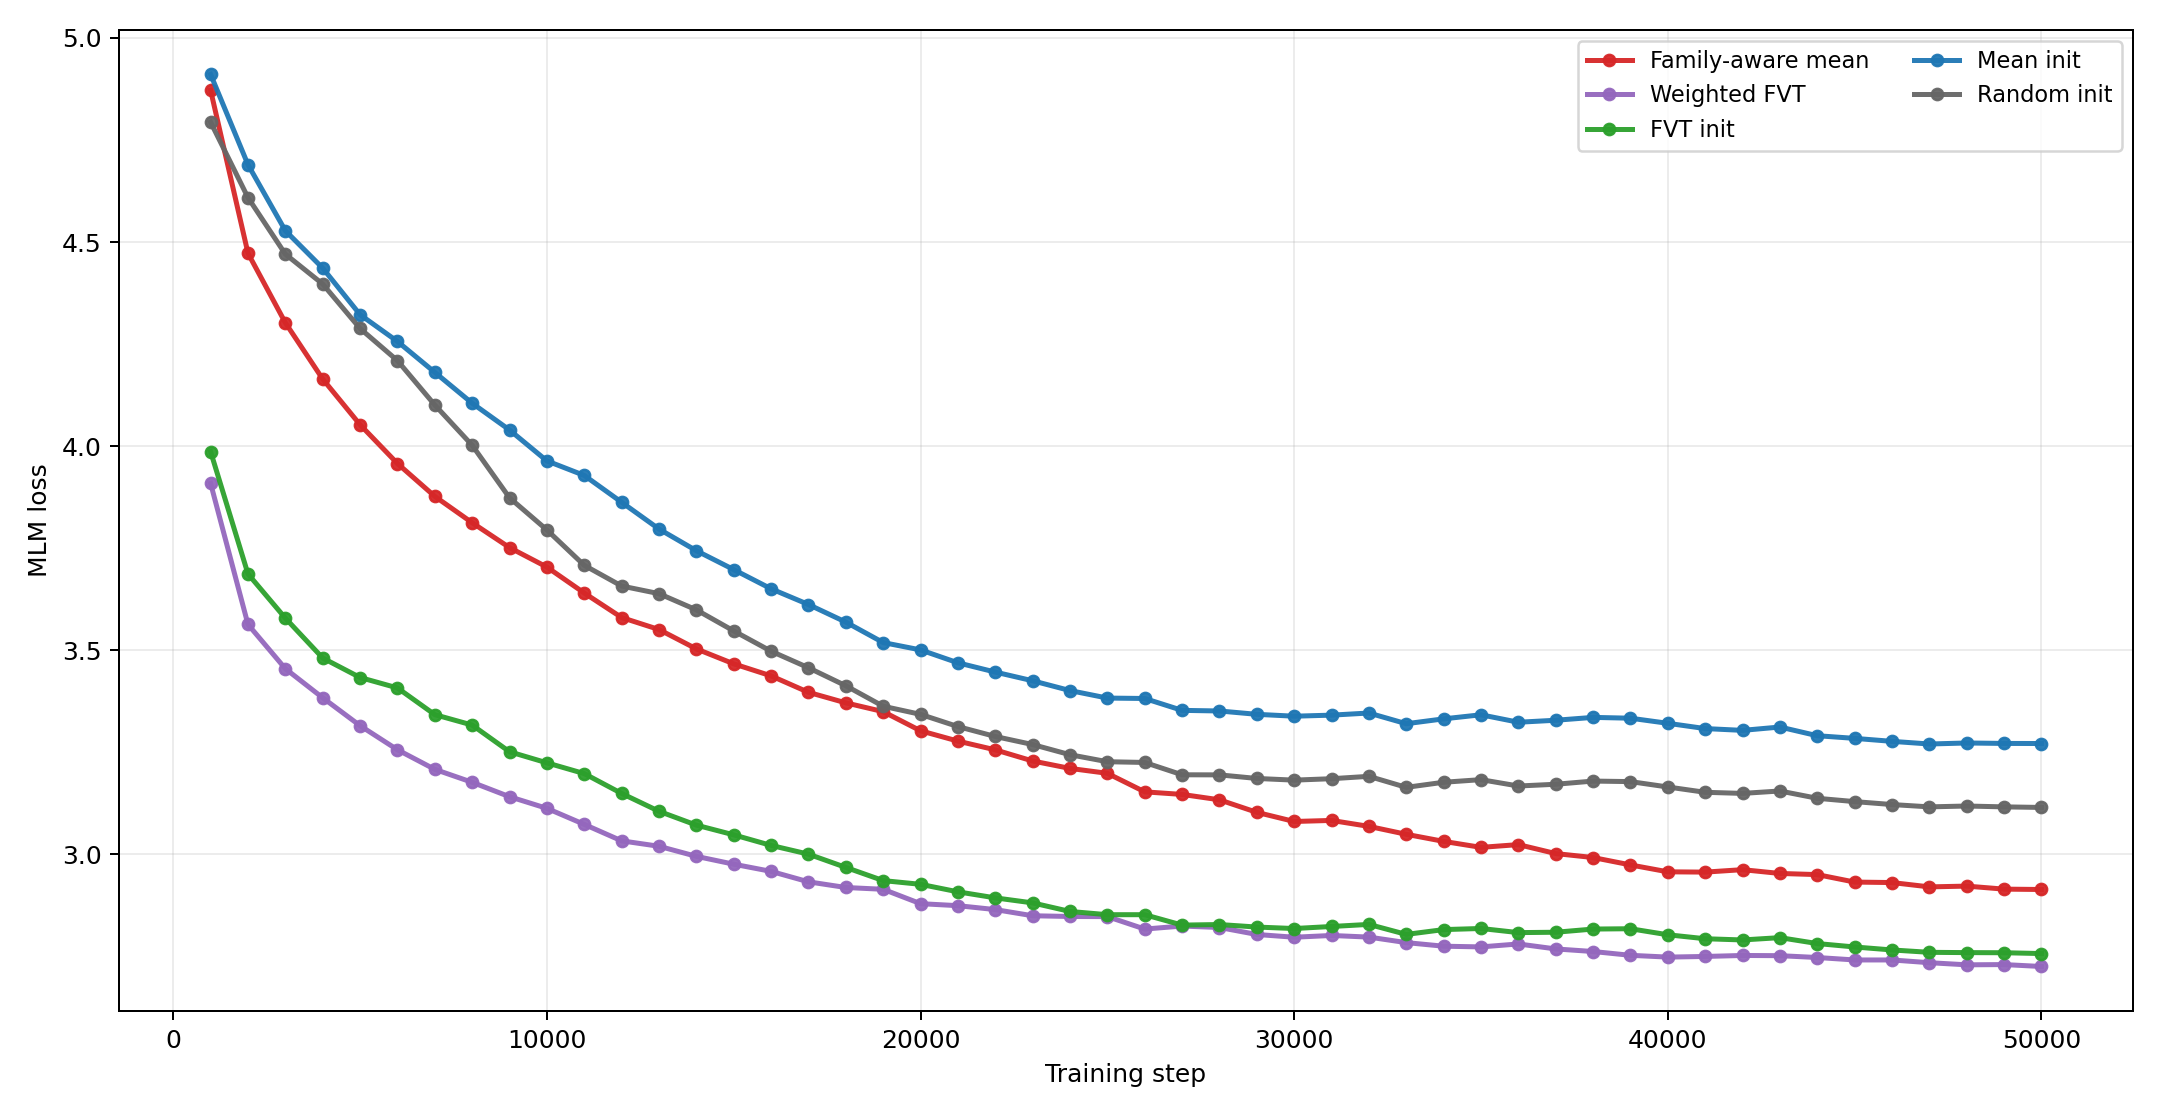
\includegraphics[width=0.82\linewidth]{convergence_5way_loss_curve.png}
\caption{5-way MLM training loss. x축=exposure-aligned step(1K grid), y축=MLM loss(낮을수록 좋음). FVT 계열 최저·\meanm\ 최악이며 순위가 수렴까지 유지된다. raw loss는 TSV에 보존되며 경계 구간에 plot-only smoothing이 포함될 수 있다.}
\label{fig:loss}
\end{figure}

\subsection{Step별 downstream 변화 (crossover)}
그림~\ref{fig:cross}는 10K$\to$50K 동안 target PPPL과 Tatoeba가 어떻게 변하는지를 다섯 방법에 대해 그린 것이다. plain \fvt\ 는 10K에 이미 최고로 출발하지만 \emph{조기 포화}해 이후 거의 개선되지 않는다. 반면 \wfvt·\famm\ 은 10K에 더 나쁘게 출발하지만 계속 개선되어 30--50K에서 \fvt\ 를 추월한다(교차 지점이 뚜렷하다). \rand·\meanm\ 은 전 구간 하위다. 즉 \textbf{정교한 초기화 prior의 이득은 학습 초반이 아니라 수렴 구간에서 드러난다} --- 짧은 진단만으로 초기화를 평가하면 잘못된 결론에 이를 수 있다. 이 crossover는 loss(그림~\ref{fig:loss})와 방향이 일치한다. 정확한 수치는 표~\ref{tab:traj}에 있다.

\begin{figure}[h]\centering
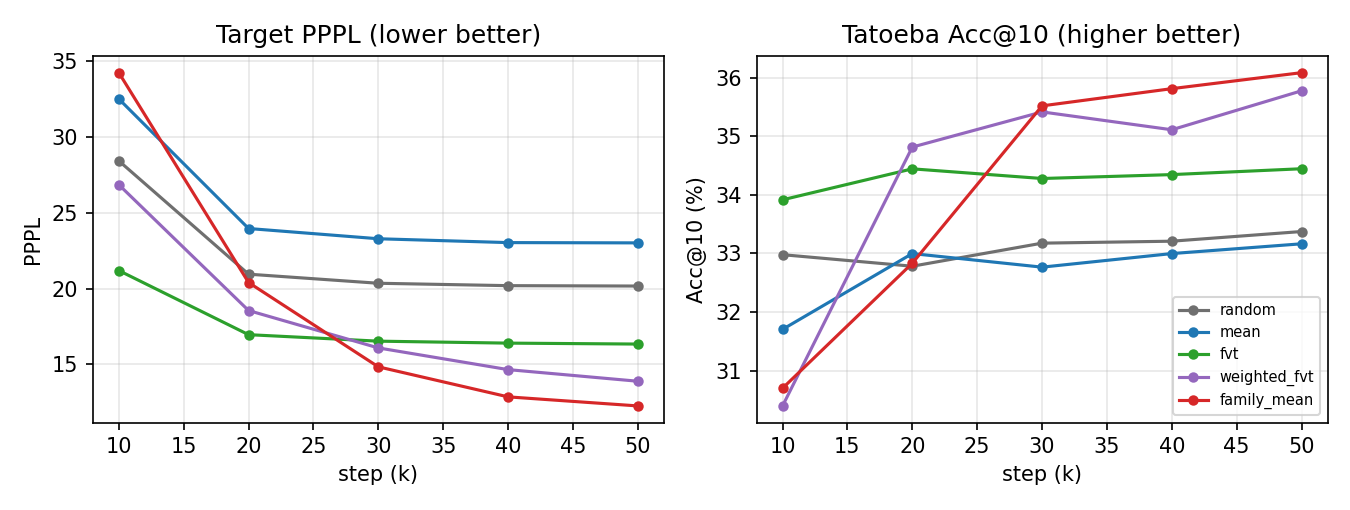
\includegraphics[width=0.95\linewidth]{crossover.png}
\caption{10K$\to$50K target 지표 궤적. 왼쪽 PPPL(낮을수록 좋음), 오른쪽 Tatoeba Acc@10(높을수록 좋음). \fvt(초록)는 조기 포화, \wfvt(보라)·\famm(빨강)은 계속 개선되어 \fvt\ 를 추월한다. \rand(회색)·\meanm(파랑)은 하위에 머문다.}
\label{fig:cross}
\end{figure}

\begin{table}[h]\centering\small
\caption{10K$\to$50K 궤적 (tail). PPPL raw, Tatoeba/Roundtrip $\times100$.}
\label{tab:traj}
\begin{tabular}{@{}lccc@{}}
\toprule
Method & PPPL (10/30/50K) & Tatoeba (10/30/50K) & Roundtrip (10/30/50K) \\
\midrule
\fvt & 21.2 / 16.5 / 16.3 & 33.9 / 34.3 / 34.4 & 3.02 / 3.24 / 3.22 \\
\wfvt & 26.9 / 16.1 / 13.9 & 30.4 / 35.4 / 35.8 & 2.85 / 3.33 / 3.38 \\
\famm & 34.2 / 14.8 / 12.3 & 30.7 / 35.5 / 36.1 & 2.61 / 3.09 / 3.16 \\
\rand & 28.4 / 20.4 / 20.2 & 33.0 / 33.2 / 33.4 & 2.61 / 2.69 / 2.67 \\
\meanm & 32.5 / 23.3 / 23.0 & 31.7 / 32.8 / 33.2 & 2.68 / 2.73 / 2.72 \\
\bottomrule
\end{tabular}
\end{table}

% =====================================================================
\section{표현 공간 분석}

\subsection{언어별·계통별 구조 형성}
문장 표현 공간에서 target 언어들이 언어별·계통별 구조를 형성하는지 본다. Target7이 모두 Latin script이므로 ``같은 문자라서 가까운가''와 ``계통이 가까워서 가까운가''를 분리해야 하며, anisotropy 때문에 raw cosine 대신 centered cosine을 쓴다. 표~\ref{tab:geo}(가장 좋은 checkpoint 50K, \fvt)에서 유사도가 \emph{같은 언어 $>$ 같은 family $>$ 같은 macro-family $>$ 다른 family} 순으로 단조 감소한다. 같은 Latin script만 공유하는 경우($-0.041$)보다 같은 family를 공유하는 경우(tail-head 0.052)가 더 가깝다 --- 즉 script 효과보다 \textbf{family/typology 효과가 더 강한 설명력}을 가지며, 같은 family가 국소 군집을 이룬다.

\begin{table}[h]\centering\small
\caption{relation bucket별 centered cosine (\fvt, 50K).}
\label{tab:geo}
\begin{tabular}{@{}lrr@{}}
\toprule
Relation & Pairs & centered cosine \\
\midrule
tail 같은 언어 & 350 & 0.455 \\
tail--tail 같은 family & 50 & 0.266 \\
tail--tail 같은 macro-family & 100 & 0.146 \\
tail--tail 다른 family & 900 & 0.074 \\
tail--head 같은 family & 1{,}050 & 0.052 \\
tail--head 다른 family·같은 Latn & 6{,}100 & $-0.041$ \\
tail--head 다른 family·다른 script & 1{,}856 & $-0.063$ \\
\bottomrule
\end{tabular}
\end{table}

\subsection{Step 변화에 따른 clustering}
그림~\ref{fig:simtrend}는 가장 잘 수렴한 \fvt\ 에서 relation bucket별 centered cosine이 10K$\to$50K로 어떻게 변하는지를 보여준다. family/language geometry는 이미 10K 시점에 대부분 형성되어 이후 거의 변하지 않는다(같은 언어 $0.458\to0.455$, 같은 family $0.274\to0.266$로 평탄). 반면 cross-lingual semantic alignment(같은 의미 src$\leftrightarrow$eng pair)는 소폭 개선 후 포화한다. 즉 \emph{쉬운 축(언어 identity, 지역)은 학습 초반에 먼저 잡히고}, 의미 정렬 같은 어려운 축은 이후 완만히 개선된다.

\begin{figure}[h]\centering
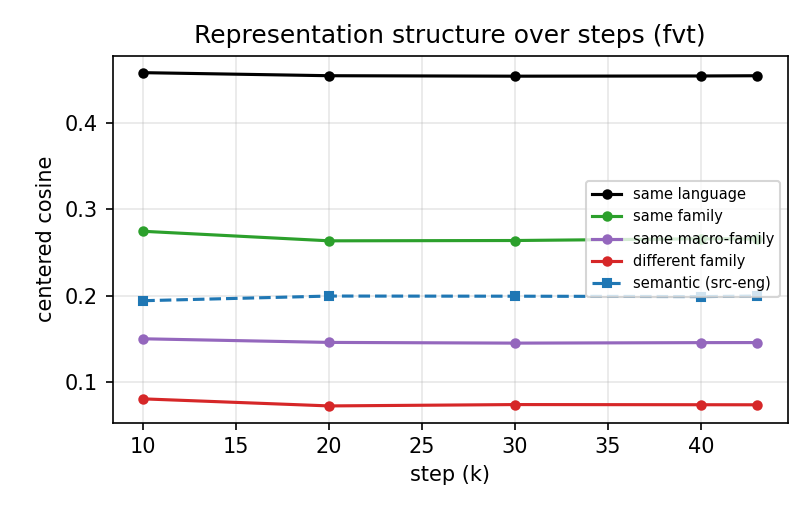
\includegraphics[width=0.62\linewidth]{sim_trend.png}
\caption{표현 구조의 step별 변화(\fvt). 언어/계통 유사도(실선)는 10K에 이미 형성되어 평탄하고, 의미 정렬(점선, src--eng)은 완만히 개선된다.}
\label{fig:simtrend}
\end{figure}

\subsection{38개 언어 2D PCA와 step별 변화}
그림~\ref{fig:map2d}는 38개 언어 subset의 문장 임베딩 평균을 2D PCA로 시각화한 것을 step 10K와 50K로 나란히 보인 것이다(색=language family, 삼각형=tail, 원=head/reference). 두 시점 모두 같은 family가 국소 군집을 이루고(Slavic \texttt{csb}와 \texttt{ces/pol} 계열, Romance \texttt{fur/lij}와 \texttt{ita/fra} 계열, Austronesian \texttt{dtp}와 \texttt{ind/msa} 계열), \texttt{dtp}·\texttt{bam}·\texttt{xav}는 주변 head가 적어 비교적 뚜렷이 분리된다. step이 진행돼도 이 군집 구조는 크게 바뀌지 않는데, 이는 \S7.2에서 관찰한 ``계통 구조는 조기에 형성되어 이후 평탄''과 일치한다. 30K 및 초기화 방법별 전체 step map은 부록~B의 그림~\ref{fig:strips}에 둔다. 각 tail centroid가 자기 계통 head 방향에 자리하는 것은 Glot500의 related-language help와 부합한다. sentence-level은 완전한 분리가 아니며 2D projection 왜곡이 있어 보조 근거로 본다.

\begin{figure}[H]\centering
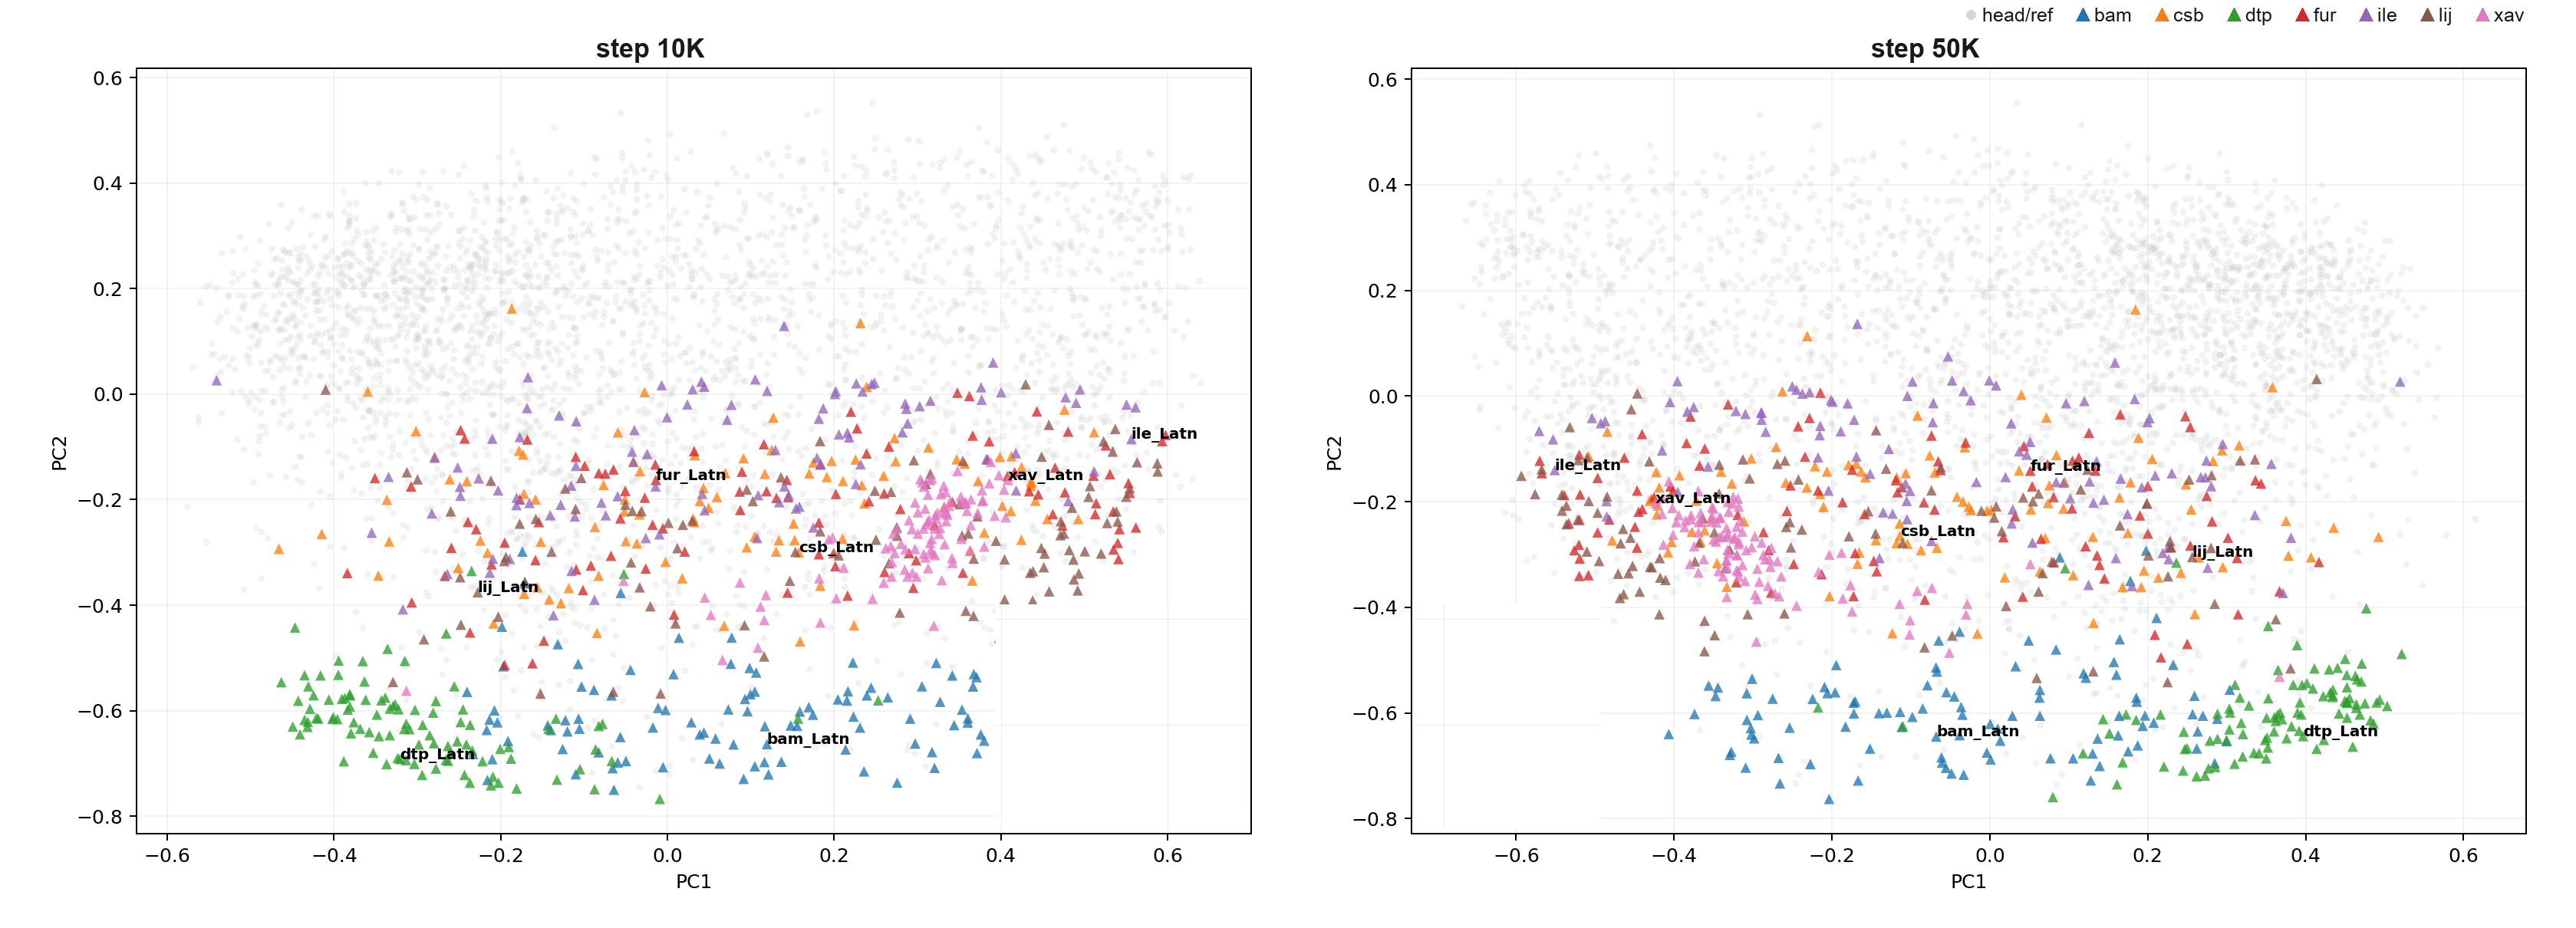
\includegraphics[width=\linewidth]{map2d_steps.png}
\caption{문장 임베딩 2D map의 step별 변화(\fvt; 왼쪽=10K, 오른쪽=50K). 색=language family, 삼각형=tail(Target7), 원=head/reference. 계통 군집 구조가 조기에 형성되어 step에 걸쳐 안정적으로 유지된다.}
\label{fig:map2d}
\end{figure}

\subsection{종합: 가장 이상적인 초기화}
표현 공간 분석과 downstream 결과를 함께 보면 핵심은 ``어떤 언어 정보를 새 embedding row에 먼저 넣는가''이다. 그림~\ref{fig:map2d}의 2D map은 모델이 유사한 언어를 가까운 표현 공간에 묶어 학습함을 보여준다. 이는 Glot500이 보고한 related-language help, 즉 주변의 관련 언어가 있을수록 저자원 언어 표현이 좋아진다는 관찰과 같은 방향이다\cite{glot500}. 다만 Table~\ref{tab:main}의 종합 순위는 계통 기반 \famm\ 하나로 정리되지 않는다. \wfvt\ 는 가장 낮은 MLM loss와 함께 PPPL head/all, Tatoeba head/all, Bible 전 group, Roundtrip 전 group에서 최고라 전체적으로 가장 강한 초기화다. \famm\ 은 tail PPPL·Tatoeba와 NER head/all에서 최고이므로 family prior는 유효하지만, 그 효과는 전체 평균보다 target tail 또는 sequence labeling 일부 지표에서 더 선명하다. plain \fvt\ 는 ``빠른 출발, 조기 포화'' 프로파일이고, NER tail·Text(EN)처럼 표면형 lexical 신호가 직접 유리한 지표에서 강하다. 결론적으로 \wfvt\ 를 종합 최선으로 보고, \famm\ 은 family prior가 필요한 target 지표에서의 보완적 강점으로 해석하는 것이 가장 방어 가능하다.

% =====================================================================
\section{결론 및 한계}

\paragraph{결론.} \texttt{xlm-roberta-base}에 Glot500식 vocabulary extension을 적용하고 새 embedding row 초기화를 다섯 방법으로 50K-step까지 통제 비교했다. (1) 확장 tokenizer는 Target7 fragmentation을 27.75\% 줄였다. (2) 같은 tokenizer·corpus에서도 초기화에 따라 50K 수렴 loss가 갈렸고, \wfvt\ 가 가장 낮은 loss로 수렴했다. (3) 50K downstream에서 \wfvt\ 는 PPPL head/all, Tatoeba head/all, Bible 전 group, Roundtrip 전 group에서 최고라 가장 강한 종합 초기화다. \famm\ 은 tail PPPL·Tatoeba와 NER head/all에서 최고이고, \fvt\ 는 NER tail과 Text(EN)에서 최고다. 즉 family prior는 유효하지만, 전체 평균적 결론은 \wfvt\ 우세로 정리하는 것이 맞다. (4) similarity 2D map과 centered cosine은 XLM-R에서 출발해 Glot500식 mixed corpus로 이어 학습한 encoder가 유사한 family 언어를 가까운 표현 공간에 연결지어 학습함을 보여준다. 이는 Glot500의 related-language help와 같은 방향이다. 따라서 가장 직접적인 결론은 새 token을 기존 subtoken 정보로 초기화하되, 균등 평균보다 표면 길이 정보를 반영한 \wfvt\ 가 가장 안정적이고, family-aware \famm\ 은 특정 target tail 및 NER 지표에서 보완적 이득을 준다는 점이다.

\paragraph{한계와 발전 방향.} 본 실험은 초기화 방법만 통제해 비교한 축소 budget study이므로 해석 범위는 Target7 Latin-script 언어와 50K training window 안으로 제한된다. 향후에는 non-Latin 및 더 넓은 계통의 target 언어로 확장해 family prior가 script가 달라져도 유지되는지 검증하고, task별 head/tail coverage와 샘플 수를 맞춘 평가셋으로 PPPL·retrieval·sequence labeling·classification 전이를 같은 기준에서 비교할 필요가 있다. 또한 10K 이전 snapshot과 50K 이후 longer run을 추가하면 family geometry가 형성되는 early phase와 downstream 수렴 구간을 분리해 볼 수 있다. \wfvt·\famm\ 은 local variant이고 단일 run이므로 multi-seed와 더 큰 budget에서 안정성을 확인해야 하며, surface FVT와 family prior를 token provenance confidence에 따라 혼합하는 ablation으로도 확장할 수 있다. 현재 family similarity 분석도 38개 language subset에 기반하므로, 더 넓은 Glot500 coverage로 확장하는 것이 다음 단계다.

% =====================================================================
\begin{thebibliography}{99}
\small
\bibitem{glot500} Imani, A. et al. (2023). Glot500: Scaling Multilingual Corpora and Language Models to 500 Languages. \textit{ACL}.
\bibitem{xlmr} Conneau, A. et al. (2020). Unsupervised Cross-lingual Representation Learning at Scale (XLM-R). \textit{ACL}.
\bibitem{spm} Kudo, T., Richardson, J. (2018). SentencePiece: A simple and language independent subword tokenizer. \textit{EMNLP (demo)}.
\bibitem{unigram} Kudo, T. (2018). Subword Regularization: Unigram Language Model. \textit{ACL}.
\bibitem{bpe} Sennrich, R. et al. (2016). Neural Machine Translation of Rare Words with Subword Units (BPE). \textit{ACL}.
\bibitem{rusttok} Rust, P. et al. (2021). How Good is Your Tokenizer? On the Monolingual Performance of Multilingual Language Models. \textit{ACL-IJCNLP}.
\bibitem{pfeifferunks} Pfeiffer, J. et al. (2021). UNKs Everywhere: Adapting Multilingual Language Models to New Scripts. \textit{EMNLP}.
\bibitem{canine} Clark, J. H. et al. (2022). CANINE: Pre-training an Efficient Tokenization-Free Encoder for Language Representation. \textit{TACL}.
\bibitem{artetxe2020} Artetxe, M. et al. (2020). On the Cross-lingual Transferability of Monolingual Representations. \textit{ACL}.
\bibitem{marchisio2023} Marchisio, K. et al. (2023). Mini-Model Adaptation: Efficiently Extending Pretrained Models to New Languages via Aligned Shallow Training. \textit{Findings of ACL}.
\bibitem{fvt} Gee, L. et al. (2022). Fast Vocabulary Transfer for Language Model Compression. \textit{EMNLP (industry)}.
\bibitem{wechsel} Minixhofer, B. et al. (2022). WECHSEL: Effective initialization of subword embeddings for cross-lingual transfer. \textit{NAACL}.
\bibitem{focus} Dobler, K., de Melo, G. (2023). FOCUS: Effective Embedding Initialization for Specializing Pretrained Multilingual Models. \textit{EMNLP}.
\bibitem{hewitt} Hewitt, J. (2021). Initializing New Word Embeddings for Pretrained Language Models. \textit{Technical note}.
\bibitem{mundra2024} Mundra, N. et al. (2024). An Empirical Comparison of Vocabulary Expansion and Initialization Approaches for Language Models. \textit{CoNLL}.
\bibitem{sakajo2025} Sakajo, H. et al. (2025). Dictionaries to the Rescue: Cross-Lingual Vocabulary Transfer for Low-Resource Languages Using Bilingual Dictionaries. \textit{Findings of ACL}.
\bibitem{lin2025} Lin, N. et al. (2025). Rethinking Vocabulary Augmentation: Addressing the Challenges of Low-Resource Languages in Multilingual Models. \textit{COLING}.
\bibitem{yamaguchi} Yamaguchi, A. et al. (2025). How Can We Effectively Expand the Vocabulary of LLMs with 0.01GB of Target Language Text? \textit{Computational Linguistics}.
\bibitem{xtreme} Hu, J. et al. (2020). XTREME: A Massively Multilingual Multi-task Benchmark. \textit{ICML}.
\bibitem{wikiann} Pan, X. et al. (2017). Cross-lingual Name Tagging and Linking for 282 Languages (WikiANN). \textit{ACL}.
\bibitem{taxi1500} Ma, C. et al. (2023). Taxi1500: A Multilingual Dataset for Text Classification in 1500 Languages.
\bibitem{tatoeba} Artetxe, M., Schwenk, H. (2019). Massively Multilingual Sentence Embeddings (Tatoeba). \textit{TACL}.
\bibitem{pppl} Salazar, J. et al. (2020). Masked Language Model Scoring. \textit{ACL}.
\bibitem{roundtrip} Dufter, P. et al. (2018). Embedding Learning Through Multilingual Concept Induction (roundtrip). \textit{ACL}.
\bibitem{bert} Devlin, J. et al. (2019). BERT: Pre-training of Deep Bidirectional Transformers. \textit{NAACL}.
\end{thebibliography}

% =====================================================================
\appendix

% =====================================================================
\section{부록 A: 보조 자료}

\subsection{Bible retrieval floor}
Bible이 다섯 방법 모두 $\sim$0.8(Acc10 $\times$100)로 붙는 것은 초기화 문제가 아니라 task 난이도 때문이다. (1) English verse 하나당 언어당 $\sim$7--8천 절 중 정답을 찾아야 해 우연 상한이 매우 낮고, (2) 절이 짧고 균질(같은 성경 구조)해 문장 벡터가 서로 매우 비슷하며, (3) 50K budget으로는 verse 수준 정밀 정렬에 도달하지 못한다. 표~\ref{tab:bible}에서 보듯 step이 지나도, 방법이 달라도 모두 floor에 머문다.

\begin{table}[h]\centering\small
\caption{Bible retrieval Acc10 ($\times100$)의 step별 값. 모든 방법이 floor.}
\label{tab:bible}
\begin{tabular}{@{}lrrrrr@{}}
\toprule
Method & 10K & 20K & 30K & 40K & 50K \\
\midrule
\rand & 0.76 & 0.79 & 0.78 & 0.79 & 0.79 \\
\meanm & 0.78 & 0.78 & 0.76 & 0.77 & 0.78 \\
\fvt & 0.78 & 0.83 & 0.83 & 0.83 & 0.84 \\
\wfvt & 0.73 & 0.86 & 0.90 & 0.83 & 0.89 \\
\famm & 0.62 & 0.70 & 0.73 & 0.71 & 0.75 \\
\midrule
XLM-R-B (참조) & \multicolumn{5}{c}{0.5} \\
\bottomrule
\end{tabular}
\end{table}

\subsection{초기화 감사 수치}
\begin{table}[h]\centering\small
\caption{초기화 구현 감사.}
\label{tab:audit}
\begin{tabular}{@{}lr@{}}
\toprule
항목 & 값 \\
\midrule
source tokenizer length & 250{,}002 \\
target tokenizer length & 366{,}666 \\
new rows & 116{,}664 \\
\verb|<mask>| id (source $\to$ target) & 250001 $\to$ 366665 \\
\verb|<mask>| copy diff & 0.0 \\
LM head tied & true \\
\bottomrule
\end{tabular}
\end{table}

% =====================================================================
\section{부록 B: 전체 결과}

\subsection{Step별 init 비교}
아래 다섯 표는 step 10K--50K 각각에서 초기화 방법별 결과를 Group(head/tail/all) 행으로 나누어 비교한 것이다. 표 형식은 본문 표~\ref{tab:main}과 동일하게 XLM-R-B/L baseline을 함께 둔다(baseline은 step과 무관하게 고정). PPPL은 raw, retrieval/roundtrip/text는 $\times100$이며, 값이 없으면 --로 표시한다. 실행 상태는 본문 상태 요약과 원자료 \path{.../11_inference/downstream_head_tail_all.tsv}의 \texttt{status} 컬럼을 따른다. Text는 현재 English만 materialized되어 tail은 --로 두고, head/all은 같은 English 값으로 둔다.

% auto-generated per-method step tables (B.1)
\begin{table}[htbp]\centering\small
\caption{초기화 \texttt{random}의 step별 target 결과 (tail; Text만 head). retrieval/roundtrip/text $\times100$, PPPL raw.}
\begin{tabular}{@{}lrrrrr@{}}
\toprule
Metric (group) & 10K & 20K & 30K & 40K & 50K \\
\midrule
PPPL $\downarrow$ & 28.4 & 21.0 & 20.4 & 20.2 & 20.2 \\
Tatoeba $\uparrow$ & 33.0 & 32.8 & 33.2 & 33.2 & 33.4 \\
Bible $\uparrow$ & 0.8 & 0.8 & 0.8 & 0.8 & 0.8 \\
NER $\uparrow$ & 44.7 & 46.6 & 46.4 & 47.0 & 48.2 \\
Roundtrip $\uparrow$ & 2.6 & 2.7 & 2.7 & 2.7 & 2.7 \\
Text(head) $\uparrow$ & 66.9 & 68.4 & 68.2 & 77.1 & 72.6 \\
\bottomrule
\end{tabular}
\end{table}

\begin{table}[htbp]\centering\small
\caption{초기화 \texttt{mean}의 step별 target 결과 (tail; Text만 head). retrieval/roundtrip/text $\times100$, PPPL raw.}
\begin{tabular}{@{}lrrrrr@{}}
\toprule
Metric (group) & 10K & 20K & 30K & 40K & 50K \\
\midrule
PPPL $\downarrow$ & 32.5 & 24.0 & 23.3 & 23.0 & 23.0 \\
Tatoeba $\uparrow$ & 31.7 & 33.0 & 32.8 & 33.0 & 33.2 \\
Bible $\uparrow$ & 0.8 & 0.8 & 0.8 & 0.8 & 0.8 \\
NER $\uparrow$ & 47.3 & 48.8 & 51.1 & 50.3 & 49.2 \\
Roundtrip $\uparrow$ & 2.7 & 2.7 & 2.7 & 2.7 & 2.7 \\
Text(head) $\uparrow$ & 78.7 & 68.2 & 71.9 & 78.8 & 68.2 \\
\bottomrule
\end{tabular}
\end{table}

\begin{table}[htbp]\centering\small
\caption{초기화 \texttt{fvt}의 step별 target 결과 (tail; Text만 head). retrieval/roundtrip/text $\times100$, PPPL raw.}
\begin{tabular}{@{}lrrrrr@{}}
\toprule
Metric (group) & 10K & 20K & 30K & 40K & 50K \\
\midrule
PPPL $\downarrow$ & 21.2 & 17.0 & 16.5 & 16.4 & 16.3 \\
Tatoeba $\uparrow$ & 33.9 & 34.4 & 34.3 & 34.3 & 34.4 \\
Bible $\uparrow$ & 0.8 & 0.8 & 0.8 & 0.8 & 0.8 \\
NER $\uparrow$ & 49.4 & 51.5 & -- & -- & 51.3 \\
Roundtrip $\uparrow$ & 3.0 & 3.3 & 3.2 & 3.2 & 3.2 \\
Text(head) $\uparrow$ & 72.4 & 79.7 & 79.7 & 79.7 & 77.4 \\
\bottomrule
\end{tabular}
\end{table}

\begin{table}[htbp]\centering\small
\caption{초기화 \texttt{weighted\_fvt}의 step별 target 결과 (tail; Text만 head). retrieval/roundtrip/text $\times100$, PPPL raw.}
\begin{tabular}{@{}lrrrrr@{}}
\toprule
Metric (group) & 10K & 20K & 30K & 40K & 50K \\
\midrule
PPPL $\downarrow$ & 26.9 & 18.6 & 16.1 & 14.7 & 13.9 \\
Tatoeba $\uparrow$ & 30.4 & 34.8 & 35.4 & 35.1 & 35.8 \\
Bible $\uparrow$ & 0.7 & 0.9 & 0.9 & 0.8 & 0.9 \\
NER $\uparrow$ & -- & -- & -- & -- & 50.6 \\
Roundtrip $\uparrow$ & 2.8 & 3.2 & 3.3 & 3.3 & 3.4 \\
Text(head) $\uparrow$ & 71.1 & 78.6 & 71.2 & 70.7 & 74.9 \\
\bottomrule
\end{tabular}
\end{table}

\begin{table}[htbp]\centering\small
\caption{초기화 \texttt{family\_mean}의 step별 target 결과 (tail; Text만 head). retrieval/roundtrip/text $\times100$, PPPL raw.}
\begin{tabular}{@{}lrrrrr@{}}
\toprule
Metric (group) & 10K & 20K & 30K & 40K & 50K \\
\midrule
PPPL $\downarrow$ & 34.2 & 20.4 & 14.8 & 12.9 & 12.3 \\
Tatoeba $\uparrow$ & 30.7 & 32.8 & 35.5 & 35.8 & 36.1 \\
Bible $\uparrow$ & 0.6 & 0.7 & 0.7 & 0.7 & 0.8 \\
NER $\uparrow$ & -- & -- & -- & -- & 55.8 \\
Roundtrip $\uparrow$ & 2.6 & 2.7 & 3.1 & 3.3 & 3.2 \\
Text(head) $\uparrow$ & 67.2 & 78.6 & 73.2 & 66.0 & 74.2 \\
\bottomrule
\end{tabular}
\end{table}


\clearpage
\subsection{Init별 step 요약}
아래 표는 B.1의 값을 초기화 방법별로 다시 묶어 10K--50K trajectory를 한눈에 보이게 한 것이다. XLM-R-B/L은 step과 무관한 고정 baseline이며, 각 지표를 head/tail/all group 행으로 나눈다. Text는 현재 English만 materialized되어 tail은 --로 두고, head/all은 같은 English 값으로 둔다.

\input{Btables_by_method.tex}

\clearpage
\subsection{초기화 방법별 step별 2D embedding map (전체)}
그림~\ref{fig:strips}는 다섯 초기화 각각에 대해 step 10K/20K/30K/40K/최종(\rand\ 43K, \meanm\ 45K, 나머지 50K)의 문장 임베딩 2D map을 4개 map 단위의 정사각형 패널로 나누어 보인 것이다. 패널 1--5는 각 초기화의 10K--40K trajectory이고, 패널 6--7은 최종 checkpoint 비교이다. 색=language family, 삼각형=tail(Target7), 원=head/reference. 모든 방법에서 계통 군집 구조가 조기에 형성되어 step에 걸쳐 안정적으로 유지된다.

\begin{figure}[p]\centering
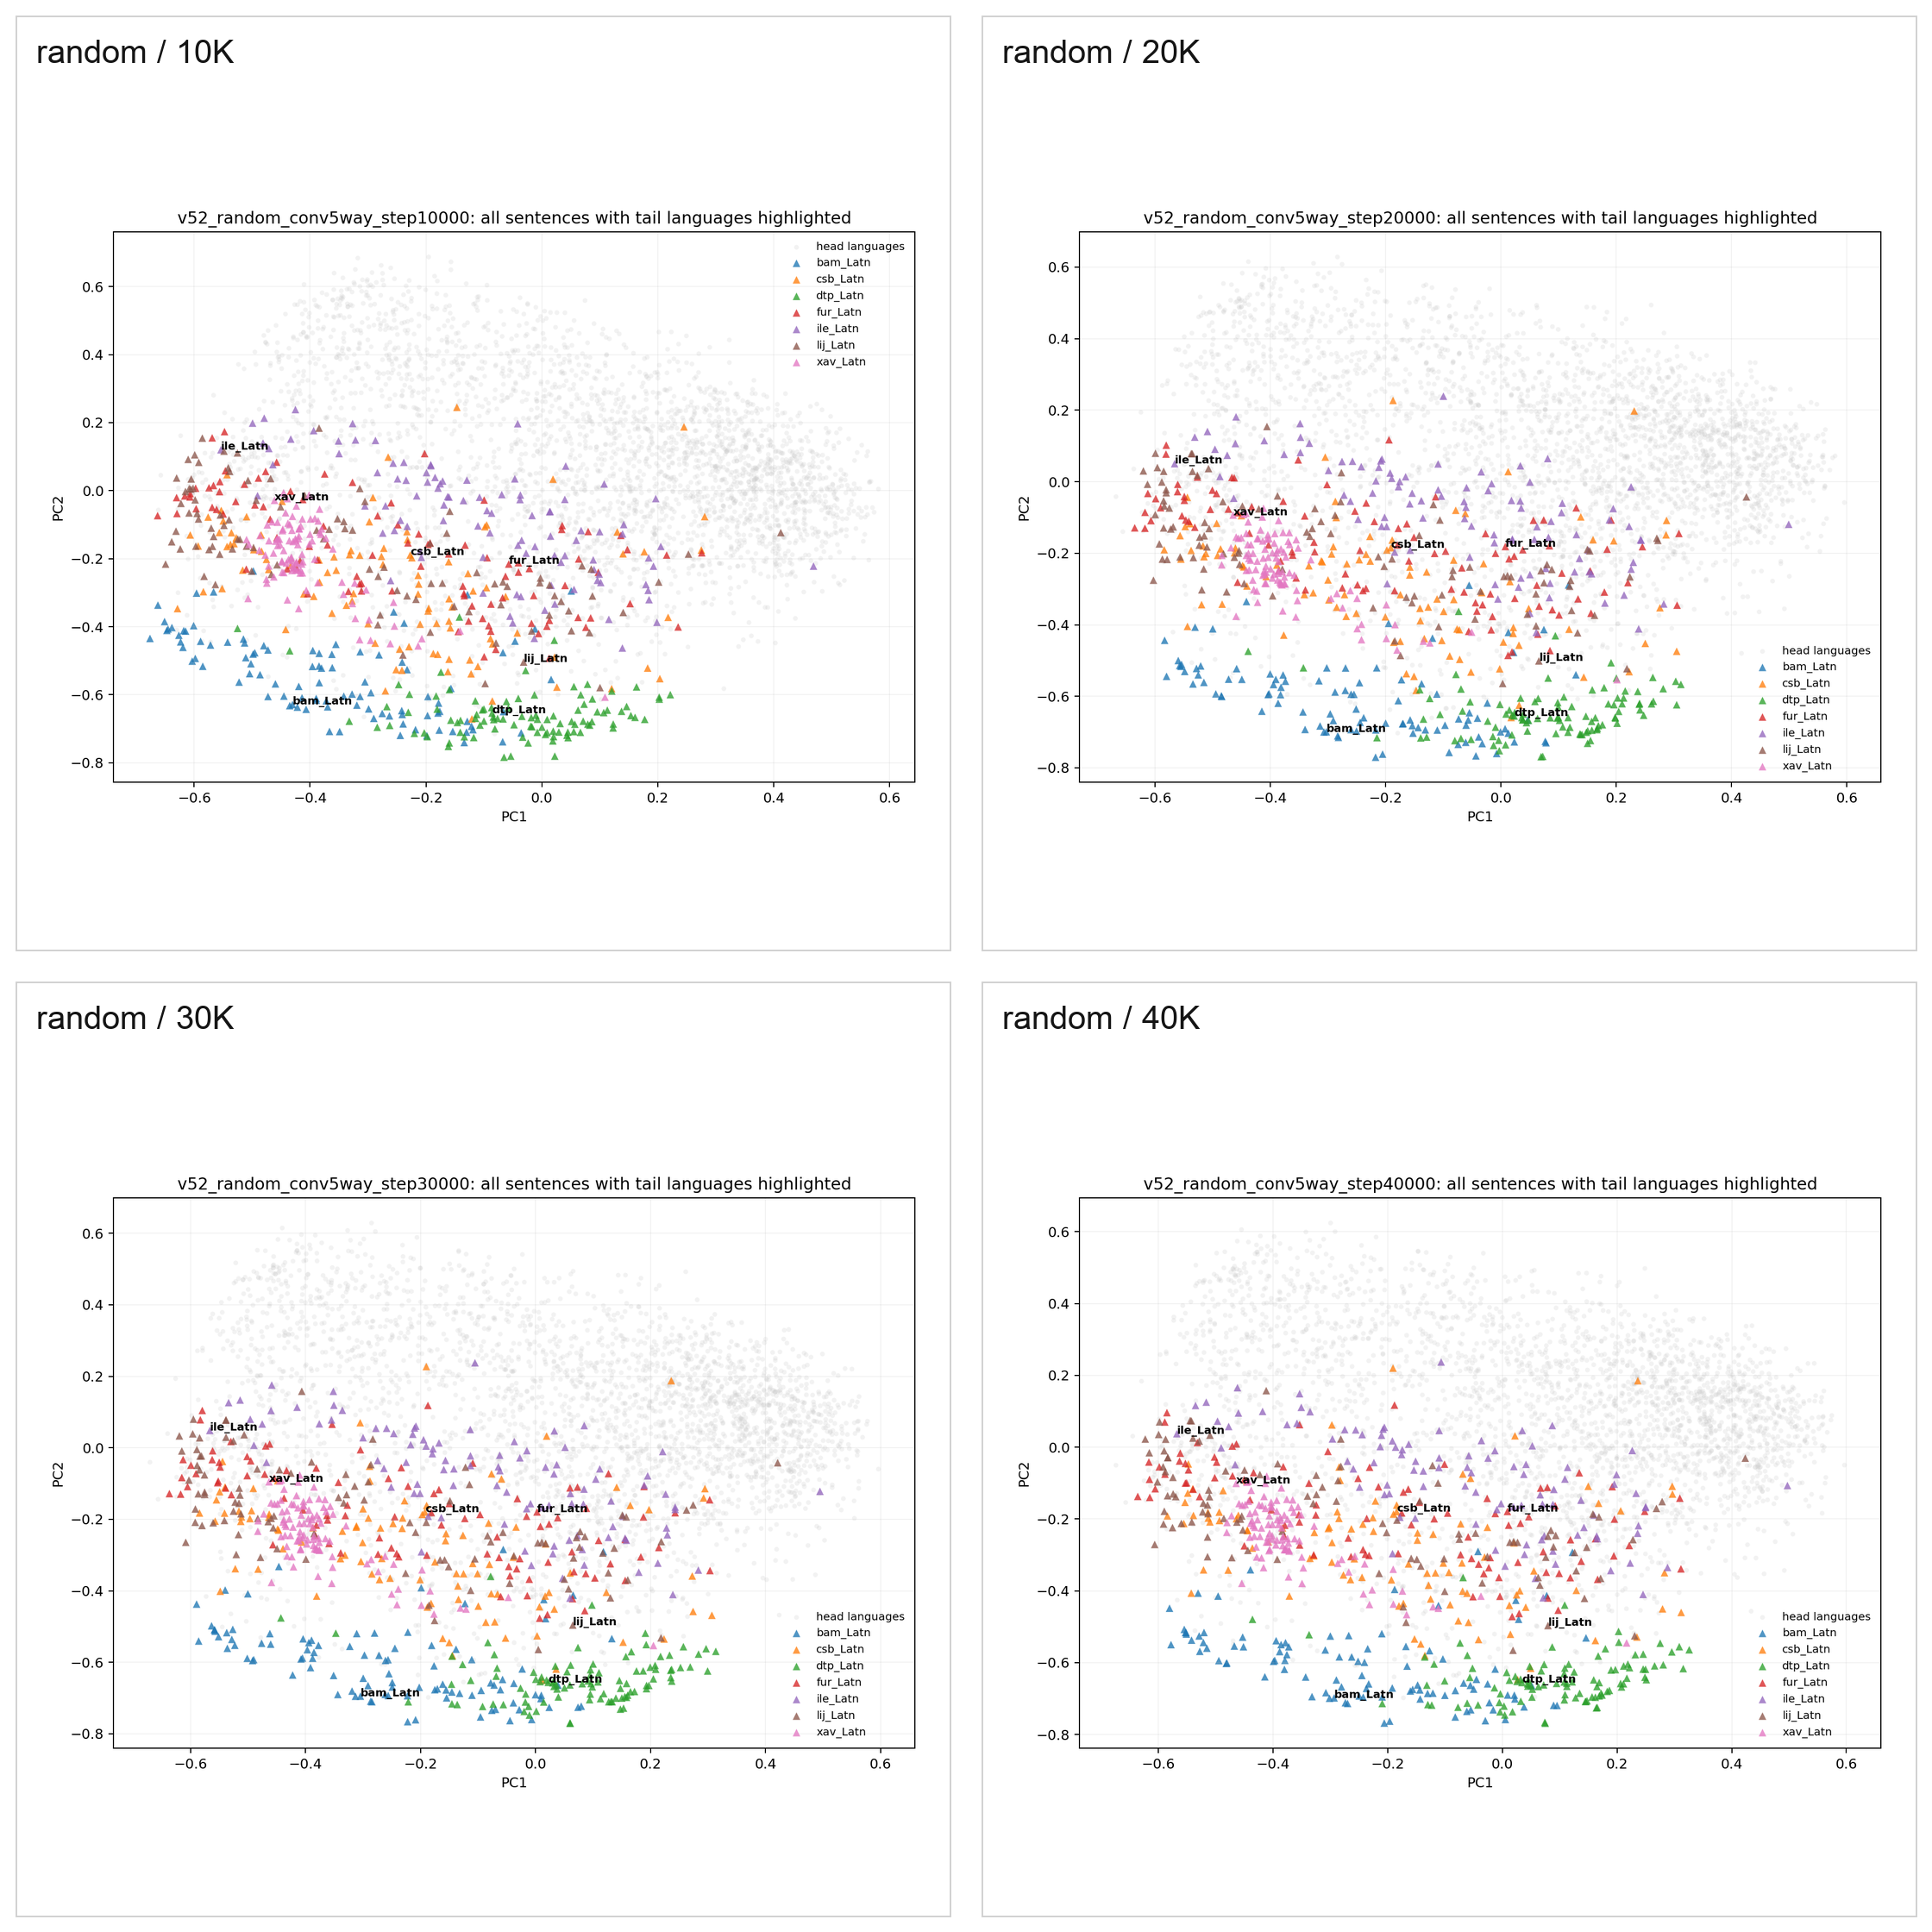
\includegraphics[width=\linewidth]{mapgrid_01.png}
\caption{초기화 방법별·step별 2D embedding map 전체(1/7): \rand\ 10K, 20K, 30K, 40K.}
\label{fig:strips}
\end{figure}

\begin{figure}[p]\ContinuedFloat\centering
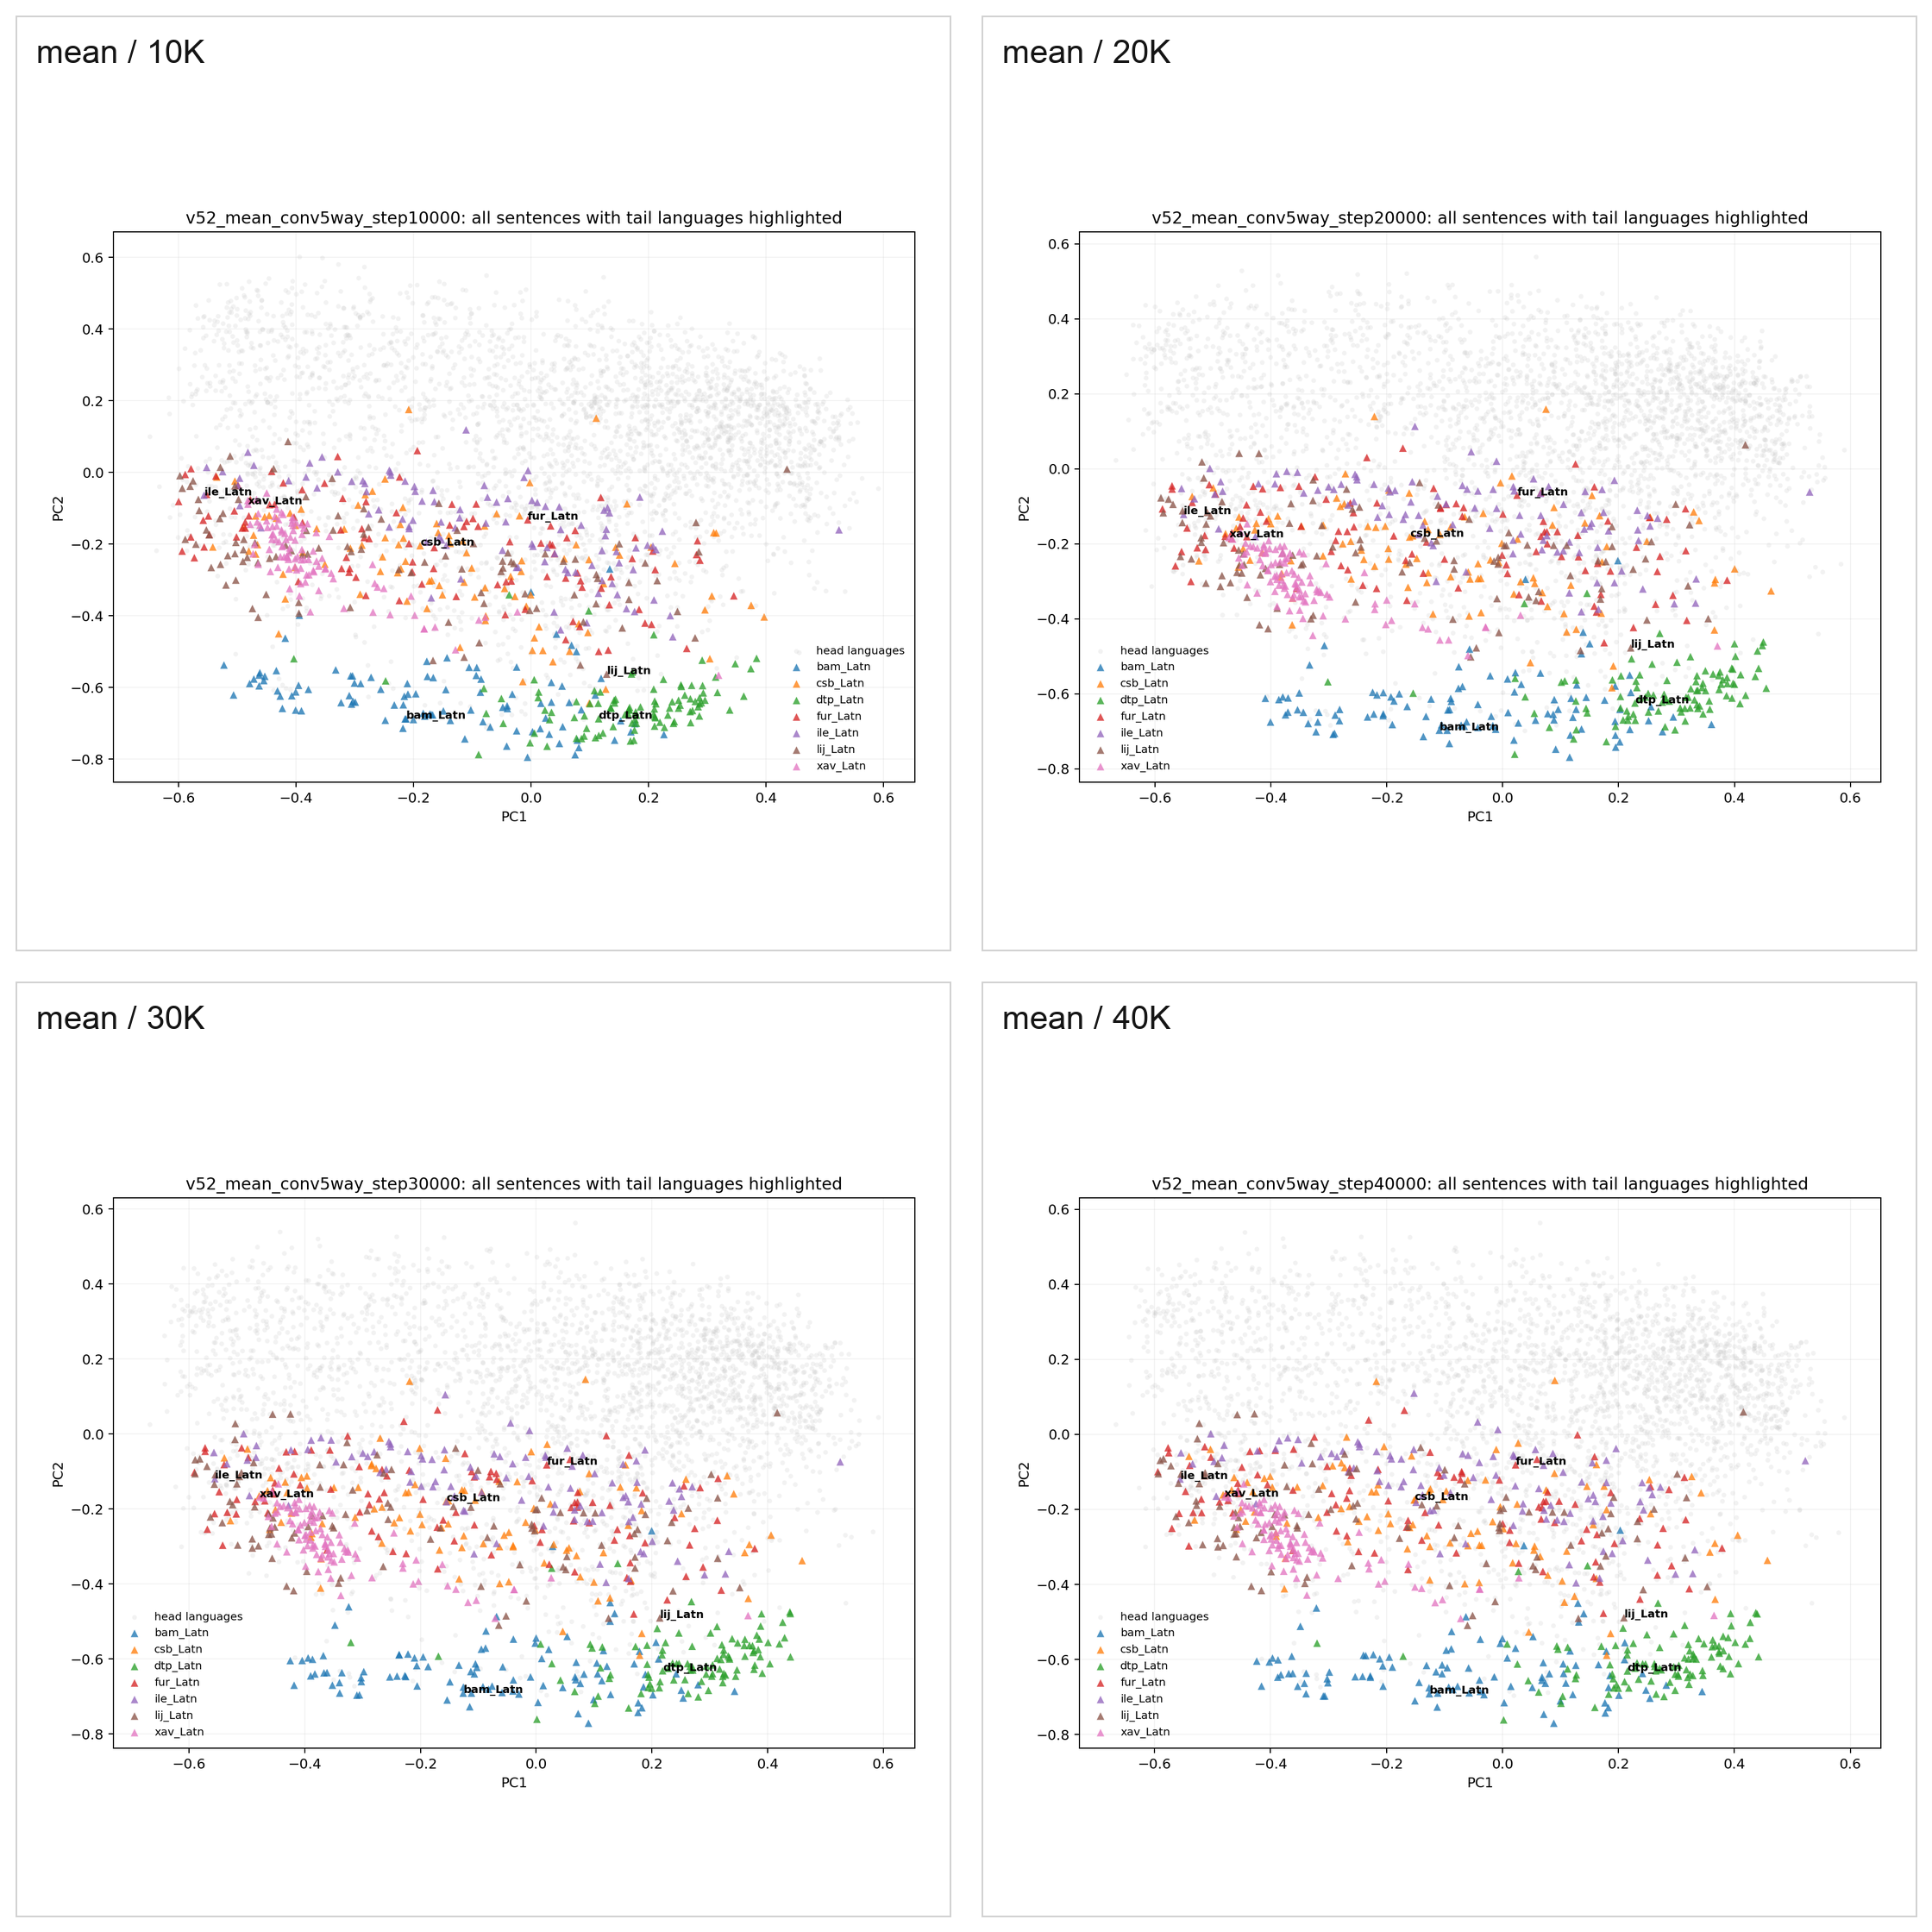
\includegraphics[width=\linewidth]{mapgrid_02.png}
\caption{초기화 방법별·step별 2D embedding map 전체(2/7): \meanm\ 10K, 20K, 30K, 40K.}
\end{figure}

\begin{figure}[p]\ContinuedFloat\centering
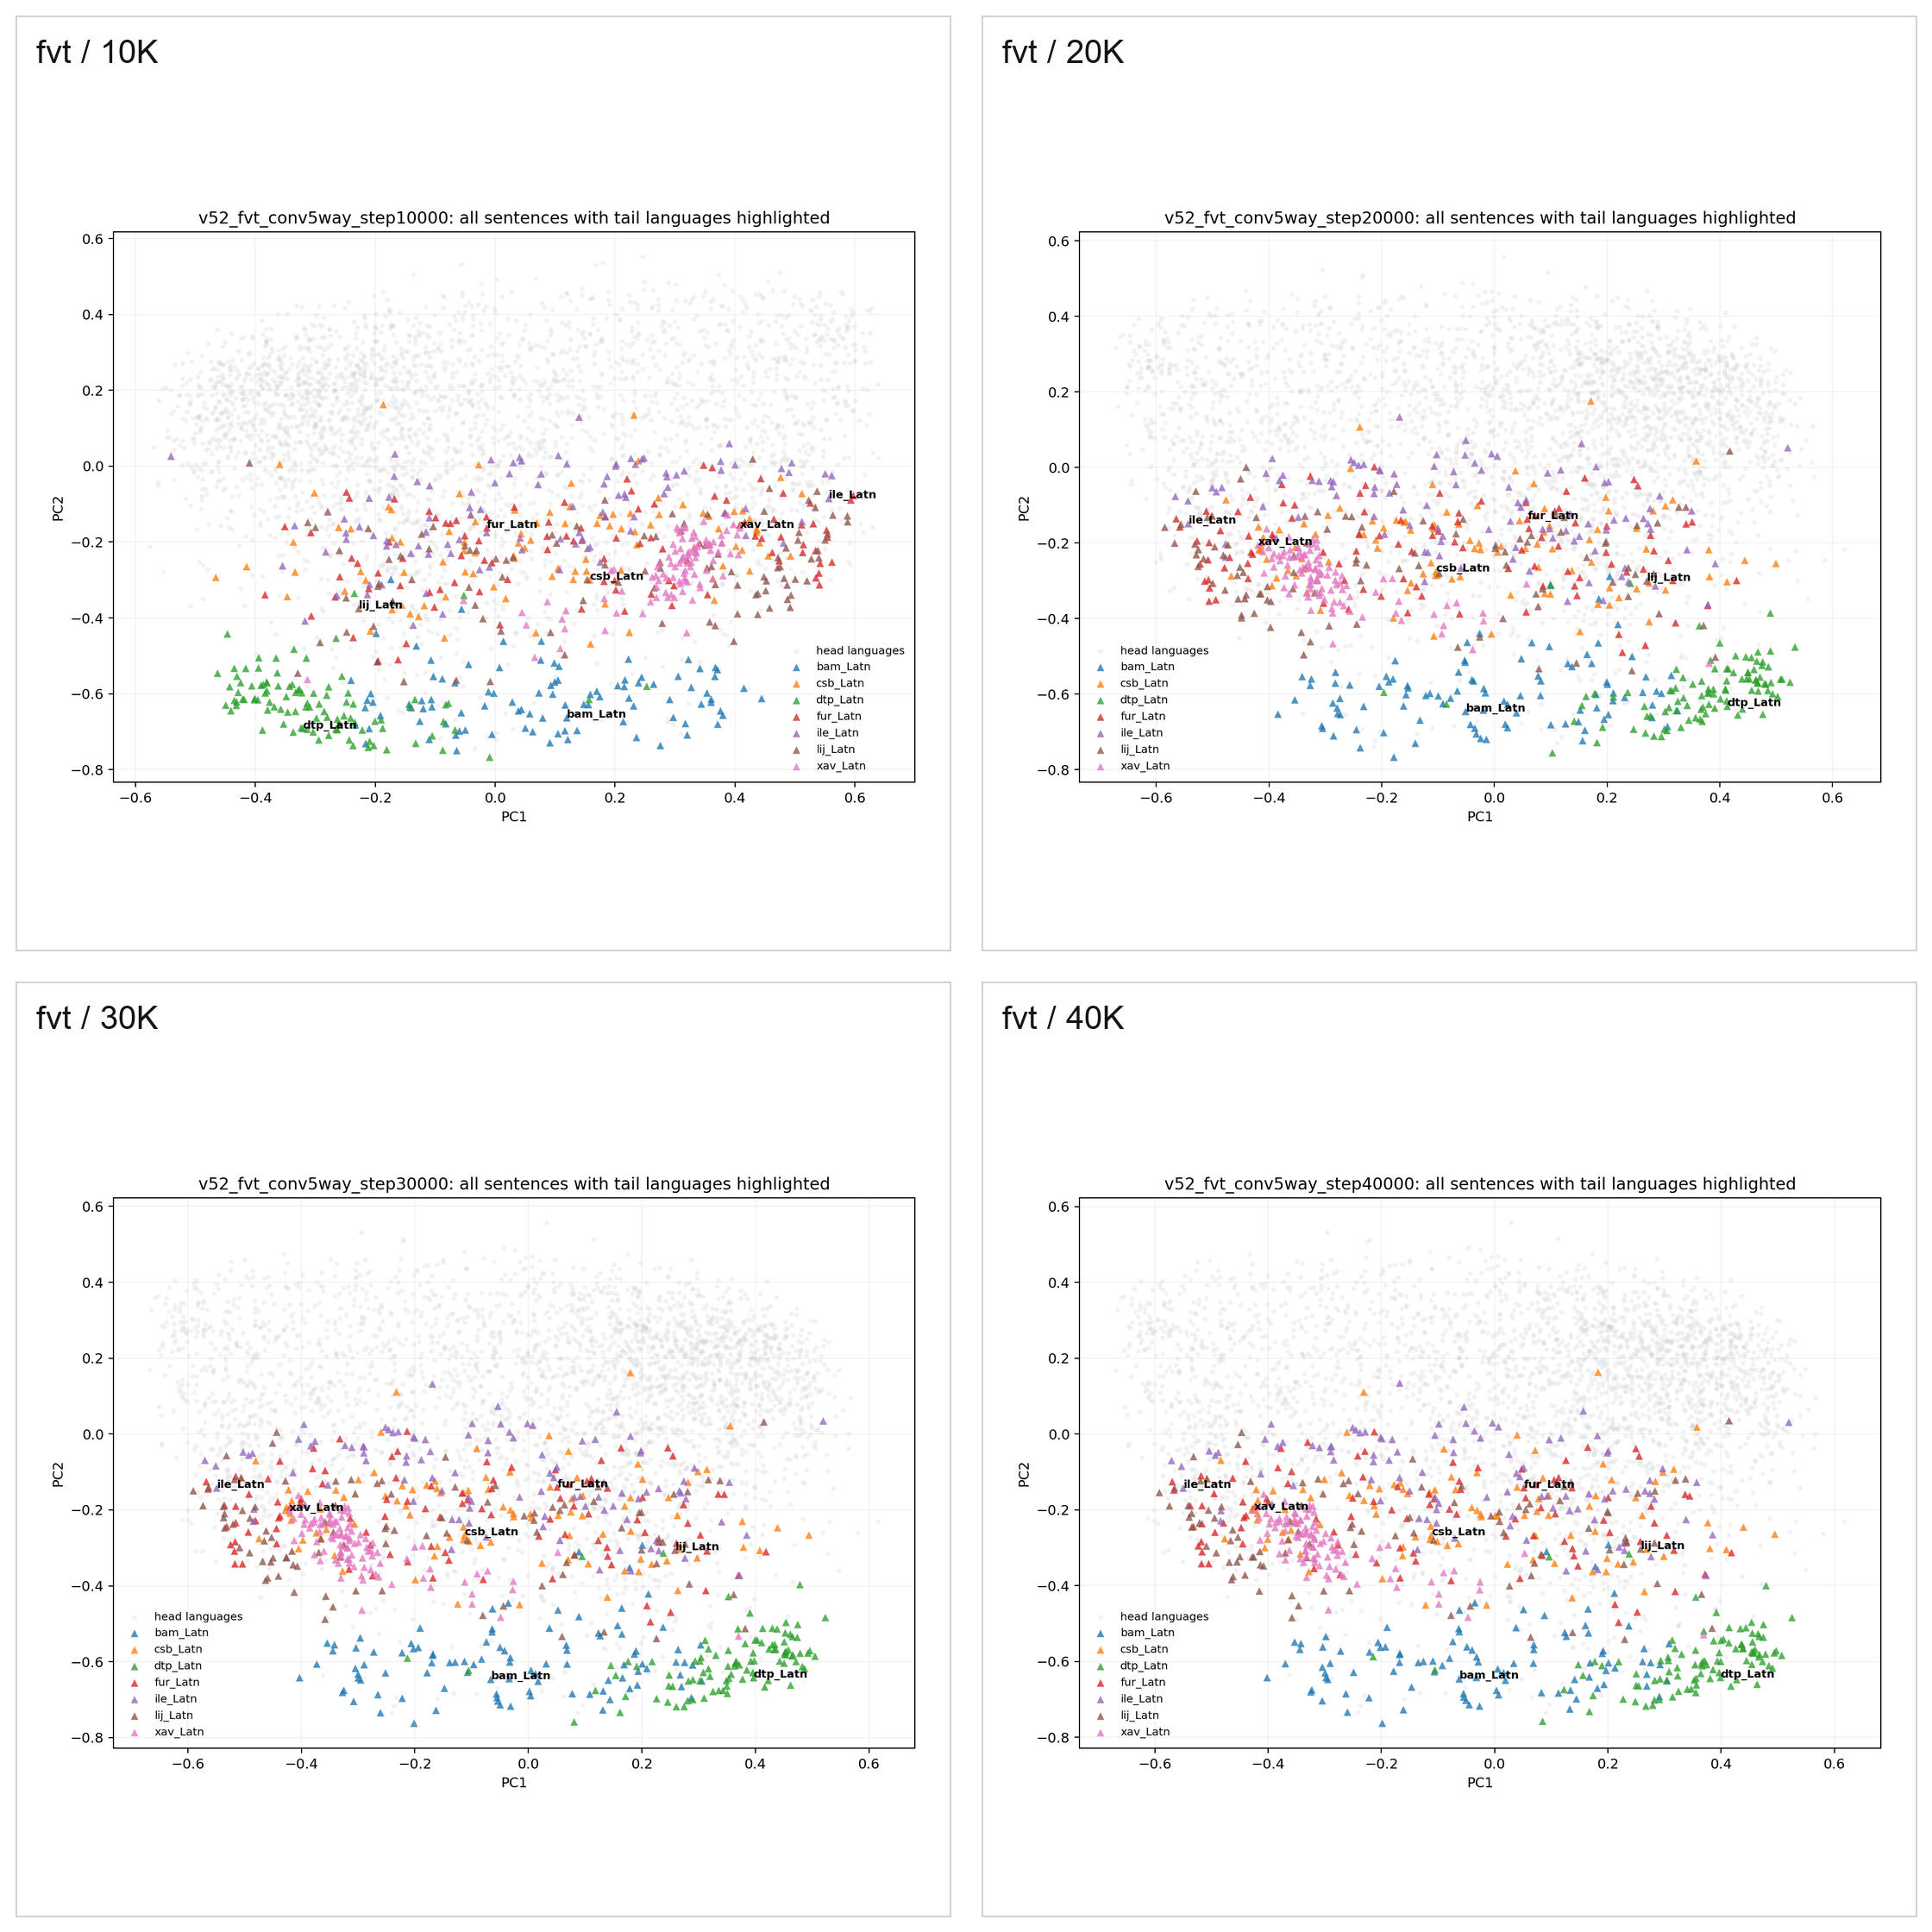
\includegraphics[width=\linewidth]{mapgrid_03.png}
\caption{초기화 방법별·step별 2D embedding map 전체(3/7): \fvt\ 10K, 20K, 30K, 40K.}
\end{figure}

\begin{figure}[p]\ContinuedFloat\centering
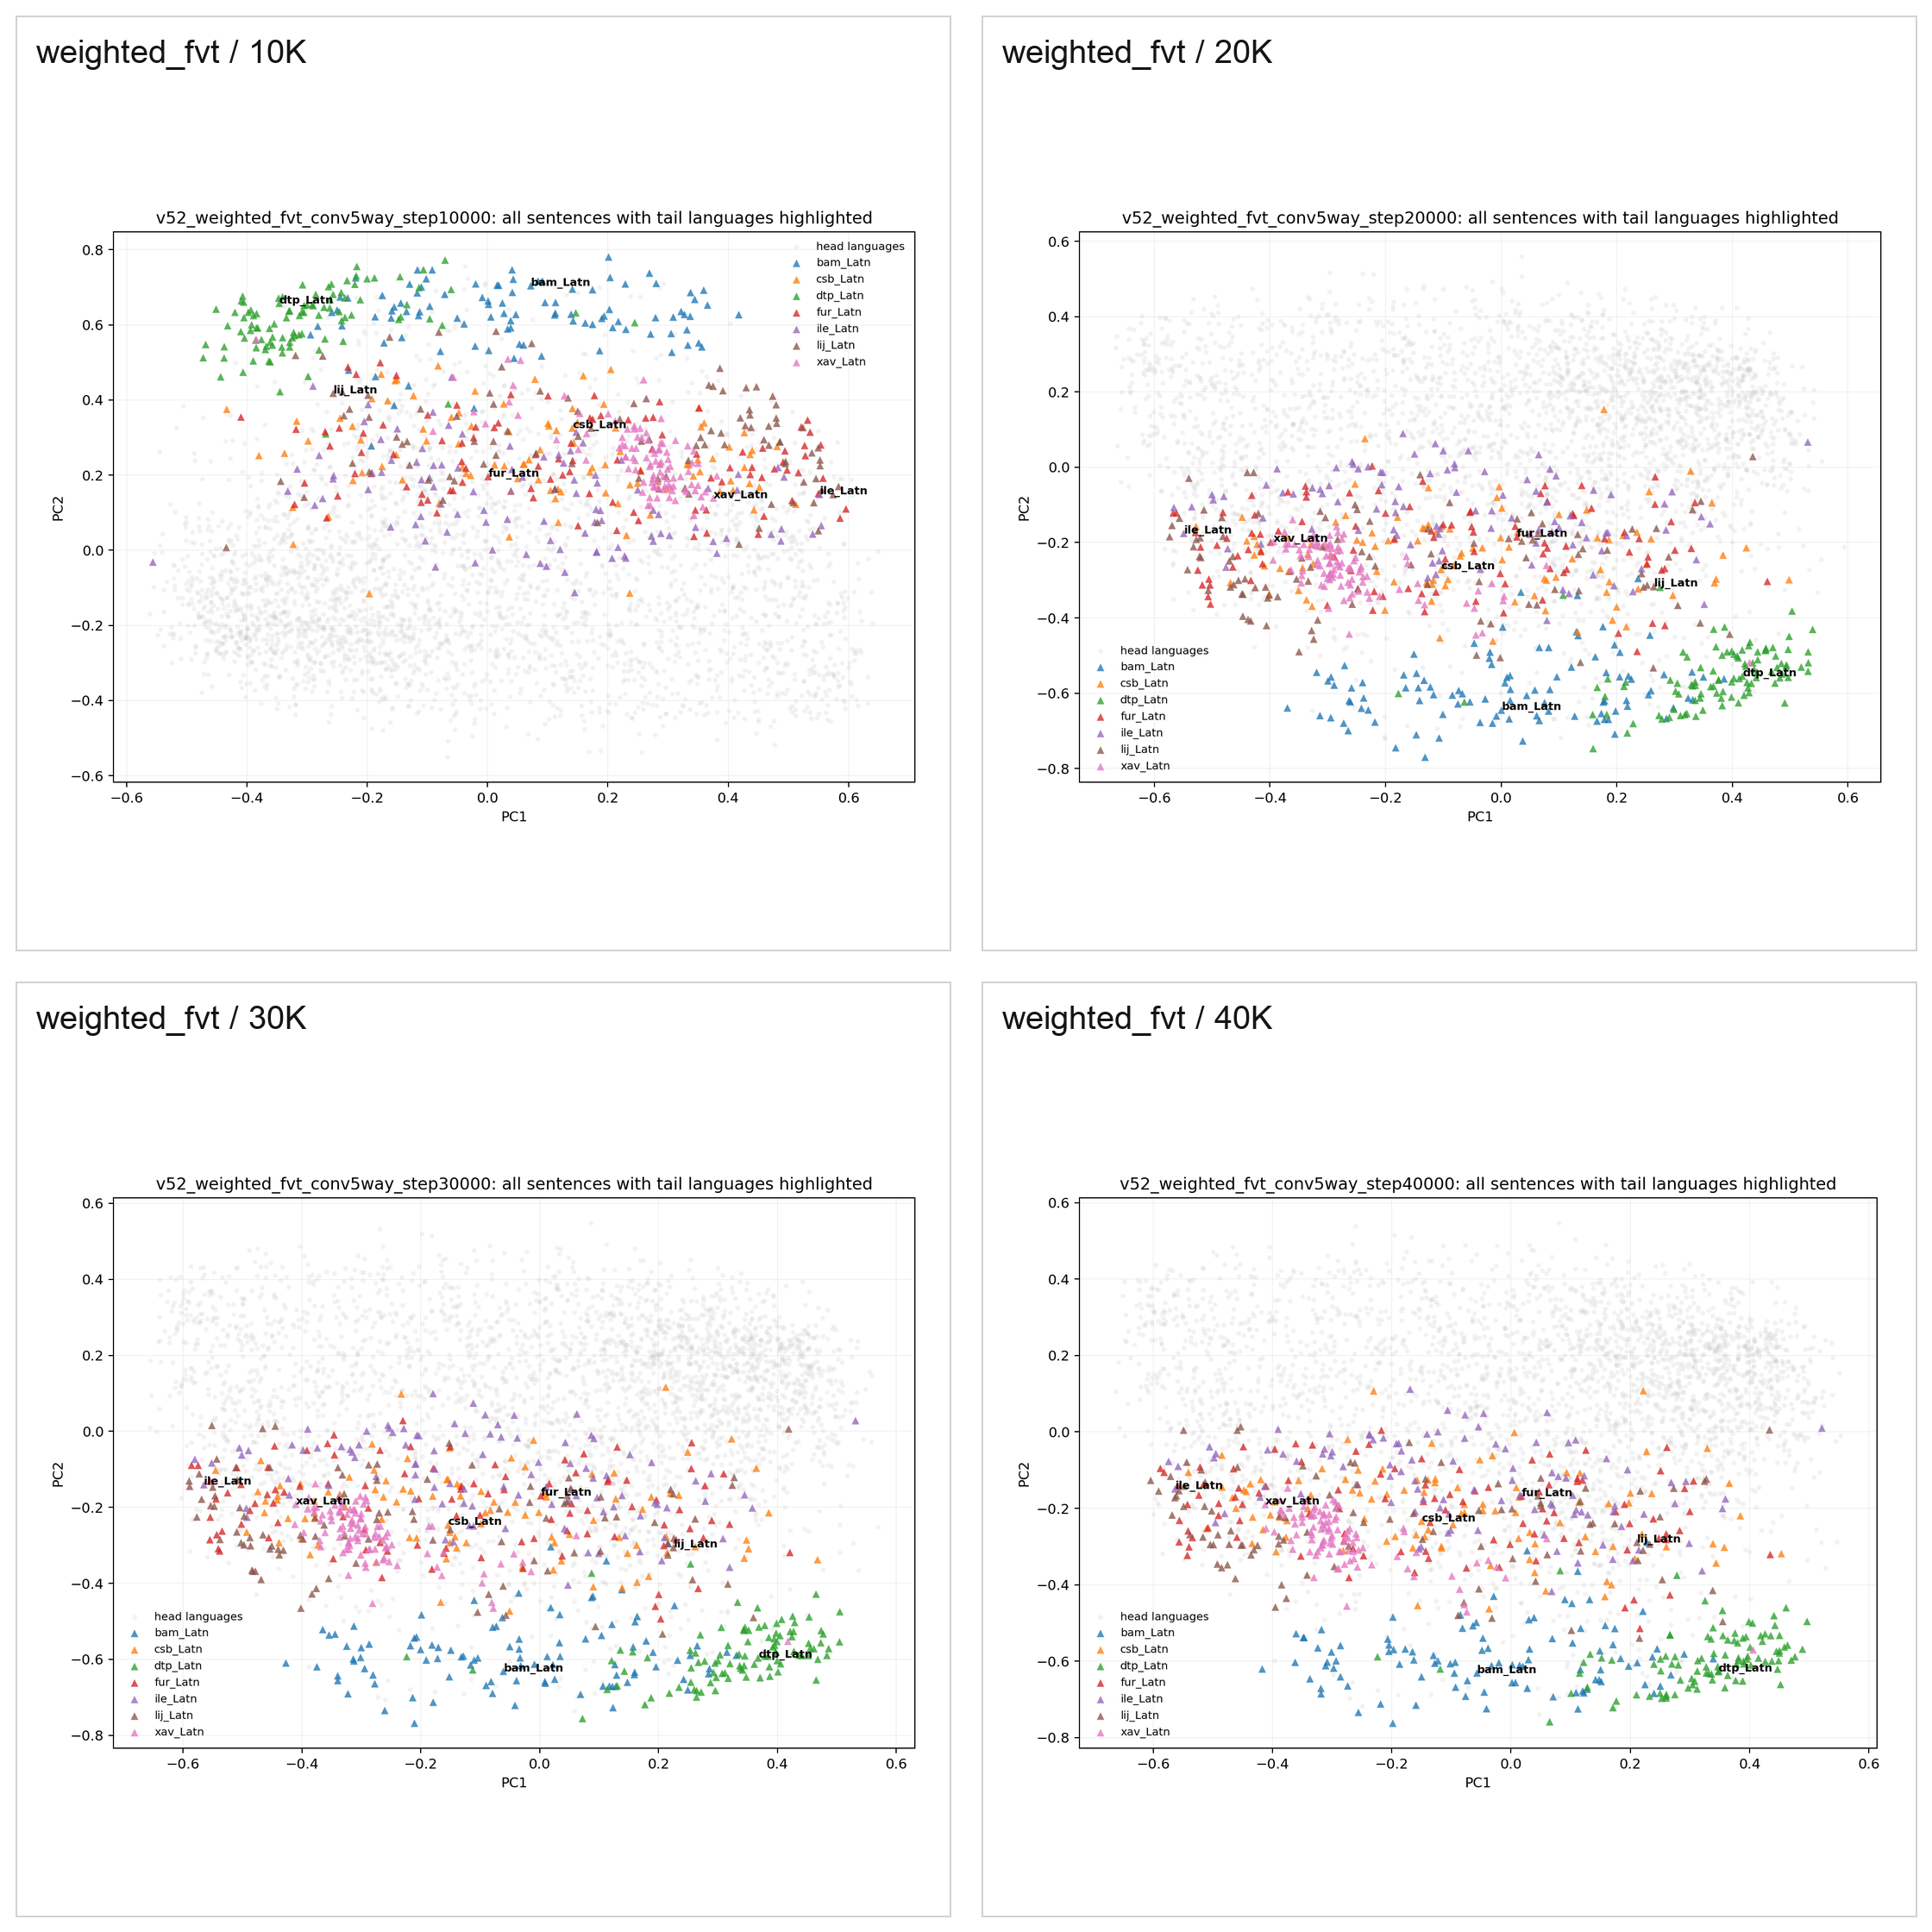
\includegraphics[width=\linewidth]{mapgrid_04.png}
\caption{초기화 방법별·step별 2D embedding map 전체(4/7): \wfvt\ 10K, 20K, 30K, 40K.}
\end{figure}

\begin{figure}[p]\ContinuedFloat\centering
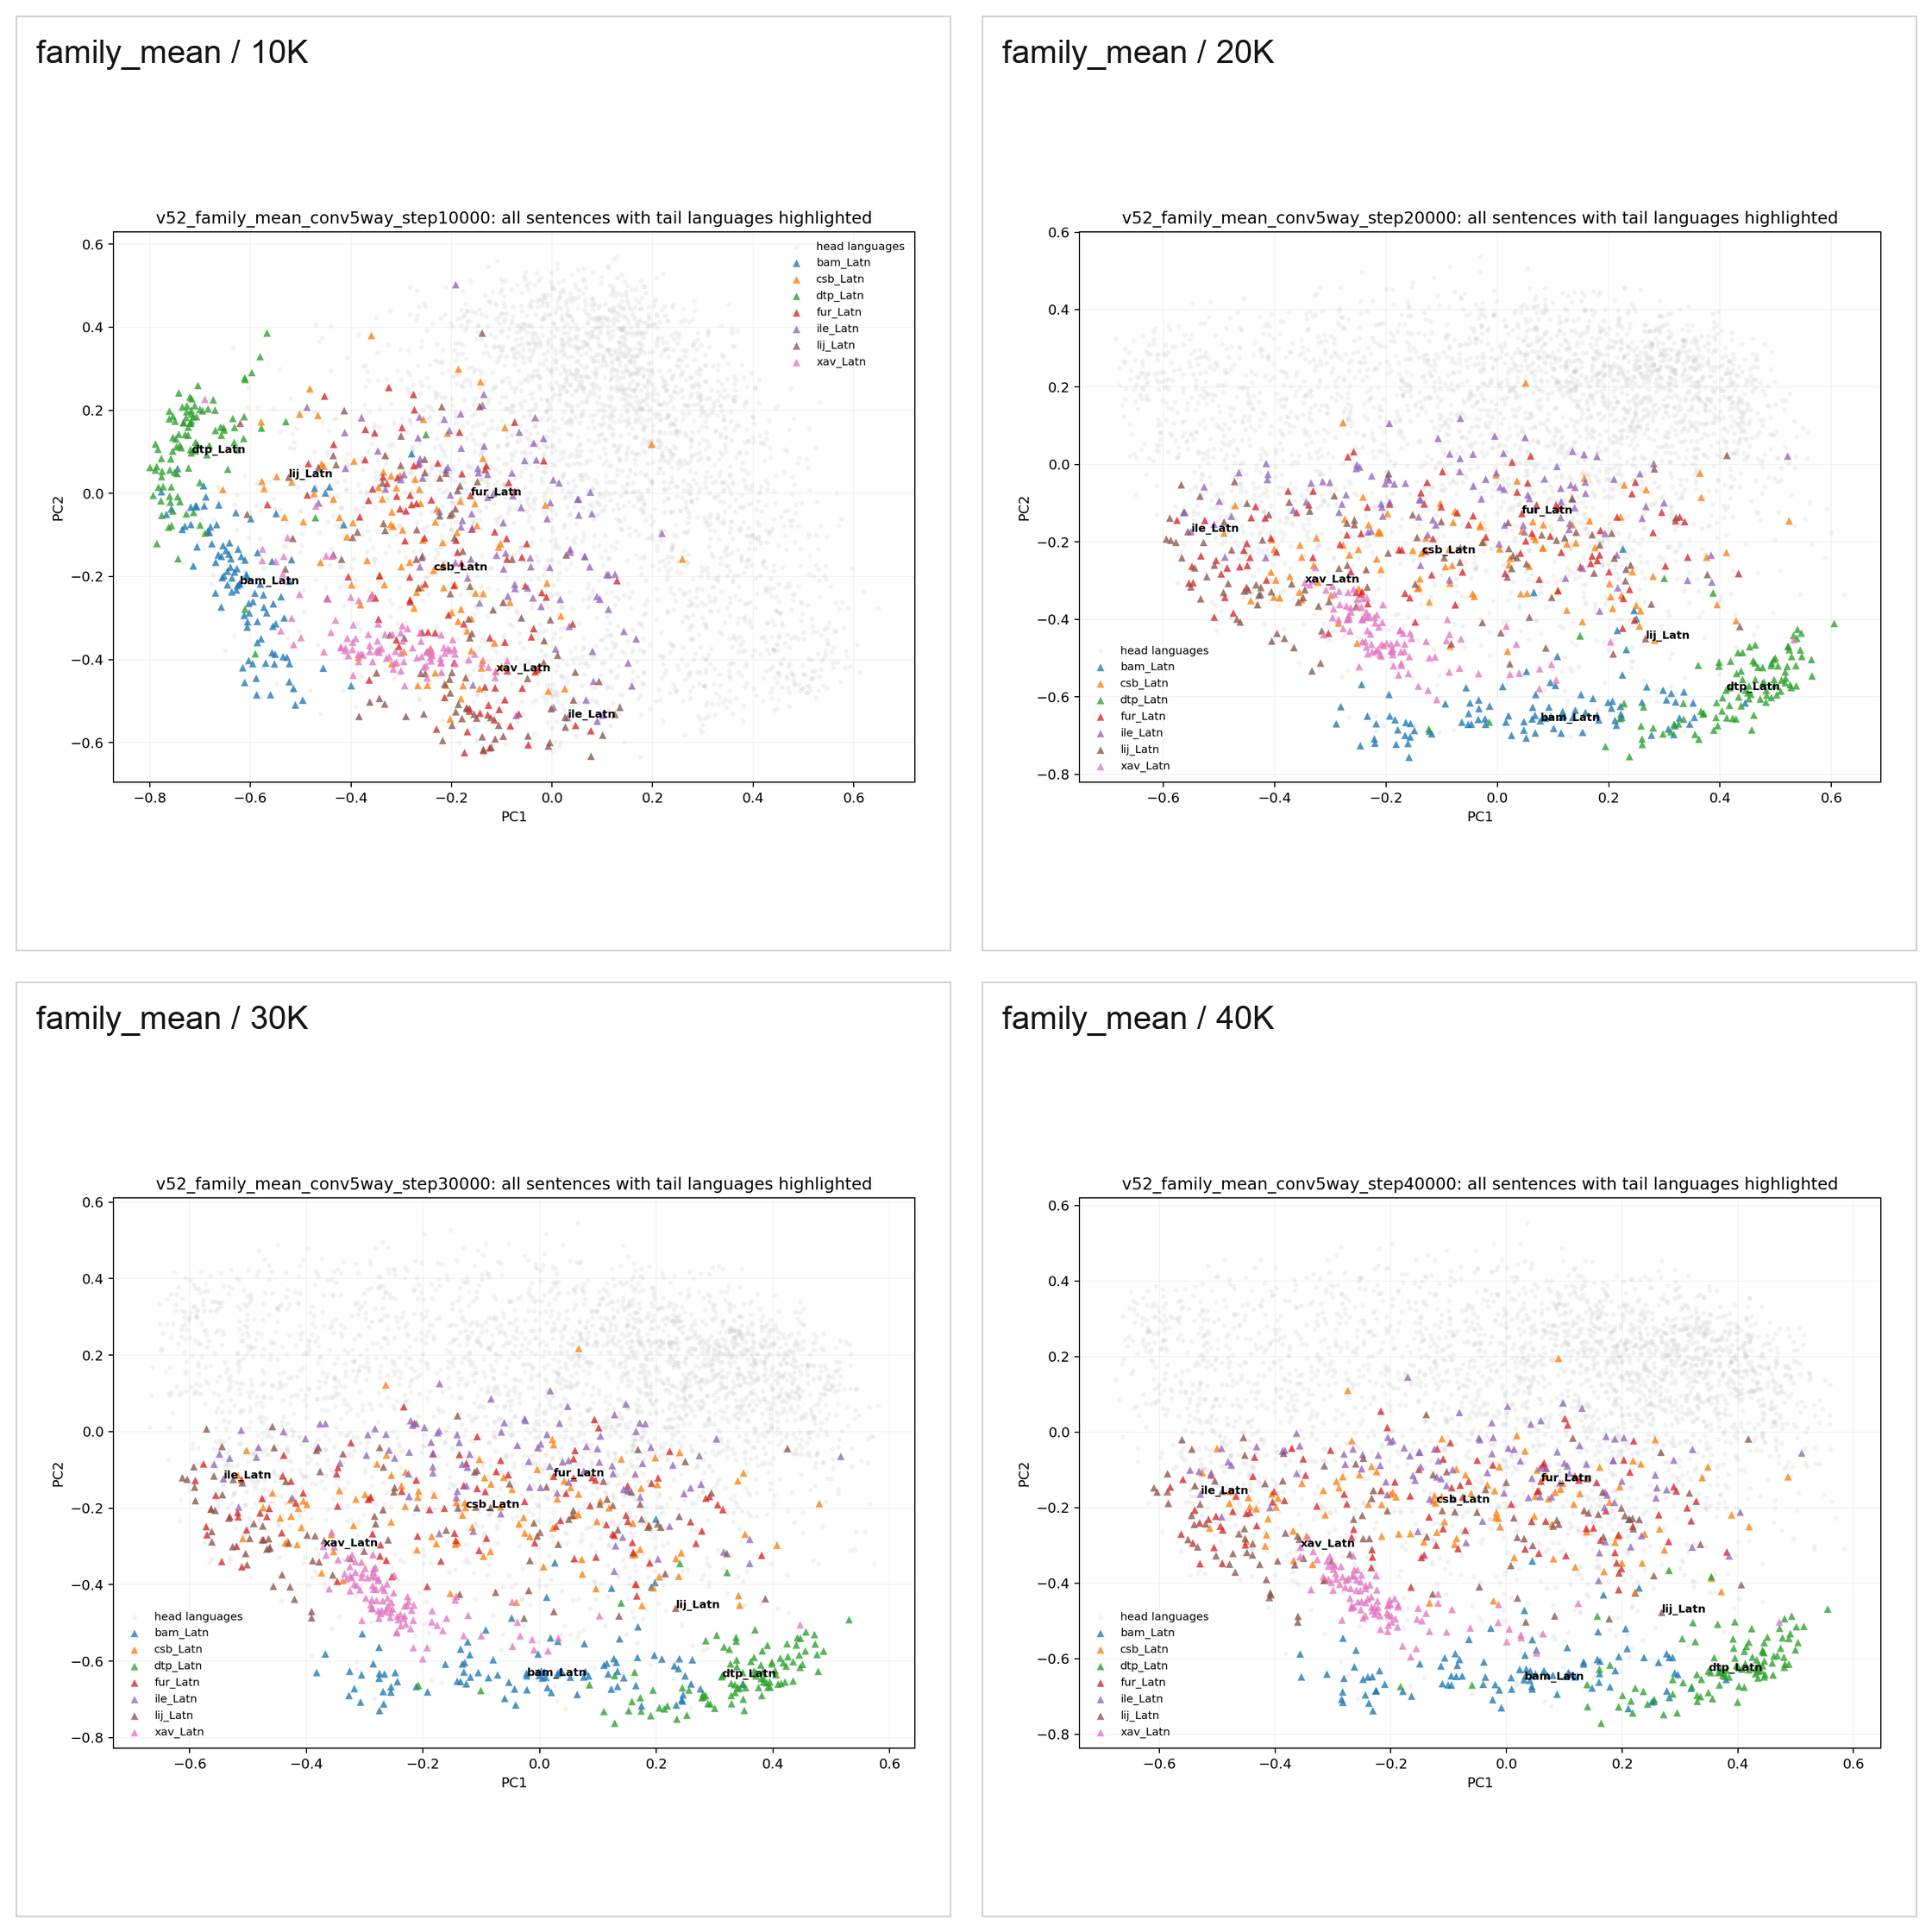
\includegraphics[width=\linewidth]{mapgrid_05.png}
\caption{초기화 방법별·step별 2D embedding map 전체(5/7): \famm\ 10K, 20K, 30K, 40K.}
\end{figure}

\begin{figure}[p]\ContinuedFloat\centering
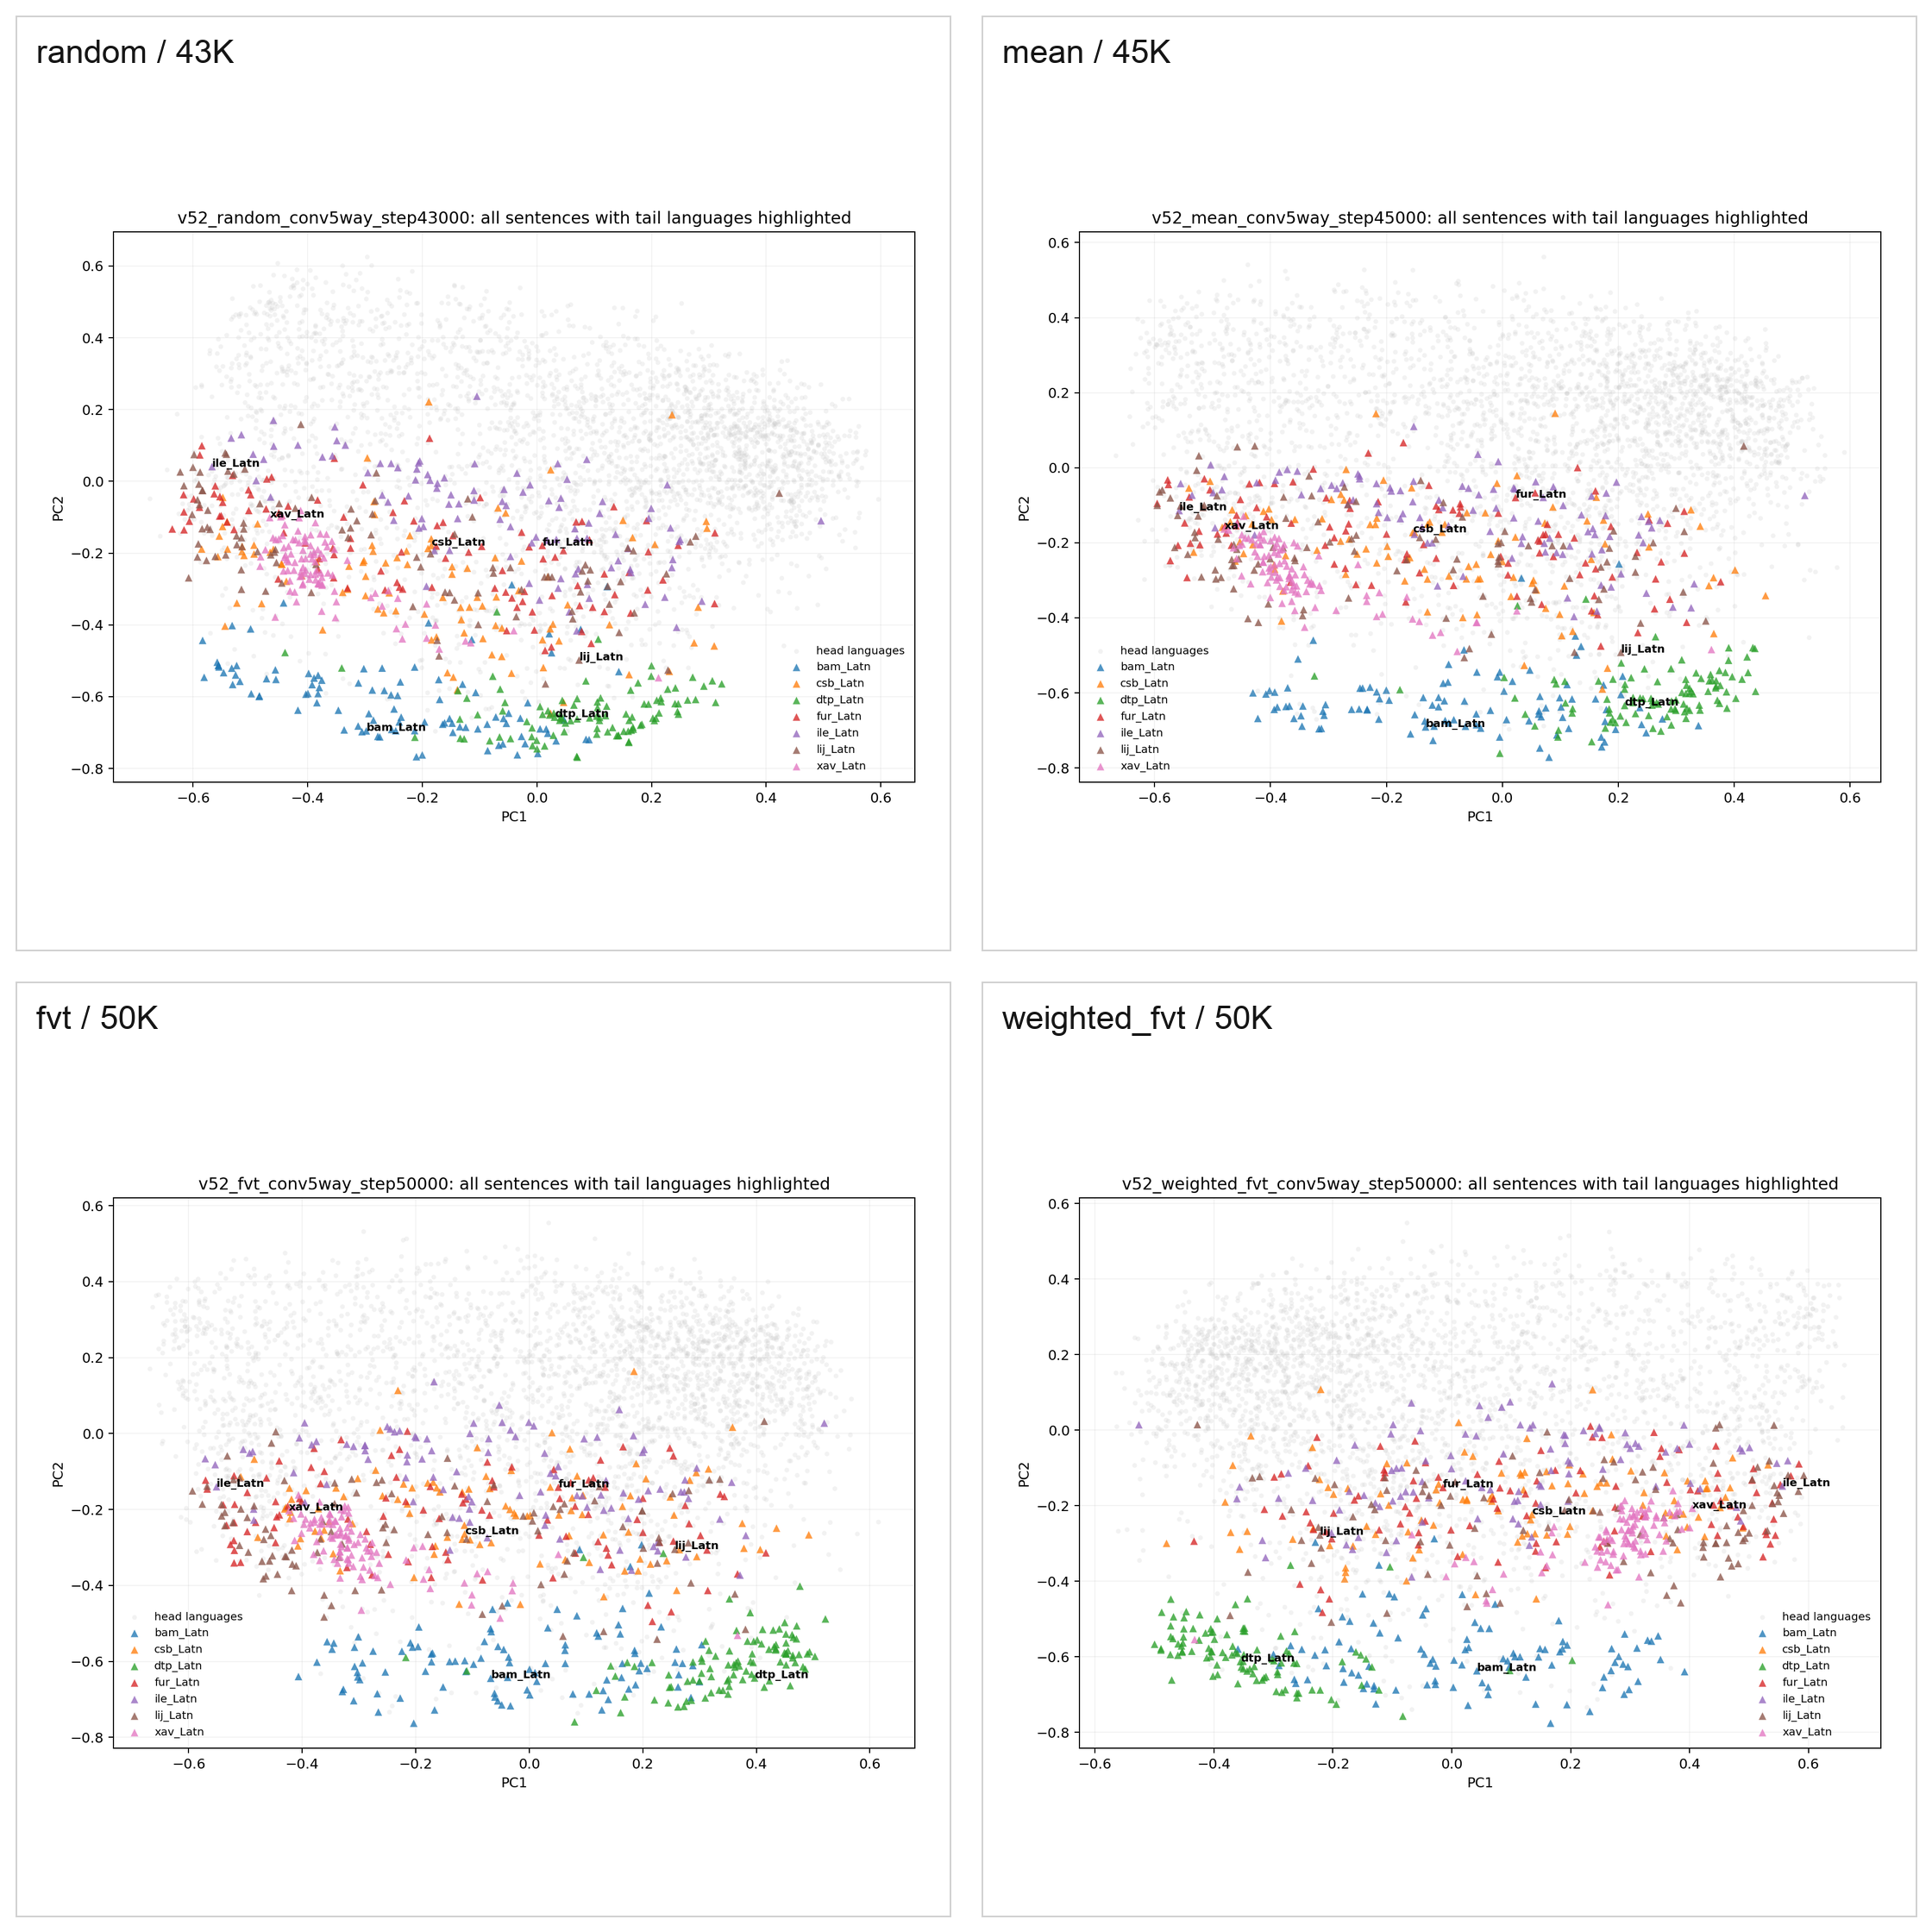
\includegraphics[width=\linewidth]{mapgrid_06.png}
\caption{초기화 방법별·step별 2D embedding map 전체(6/7): \rand\ 43K, \meanm\ 45K, \fvt\ 50K, \wfvt\ 50K.}
\end{figure}

\begin{figure}[p]\ContinuedFloat\centering
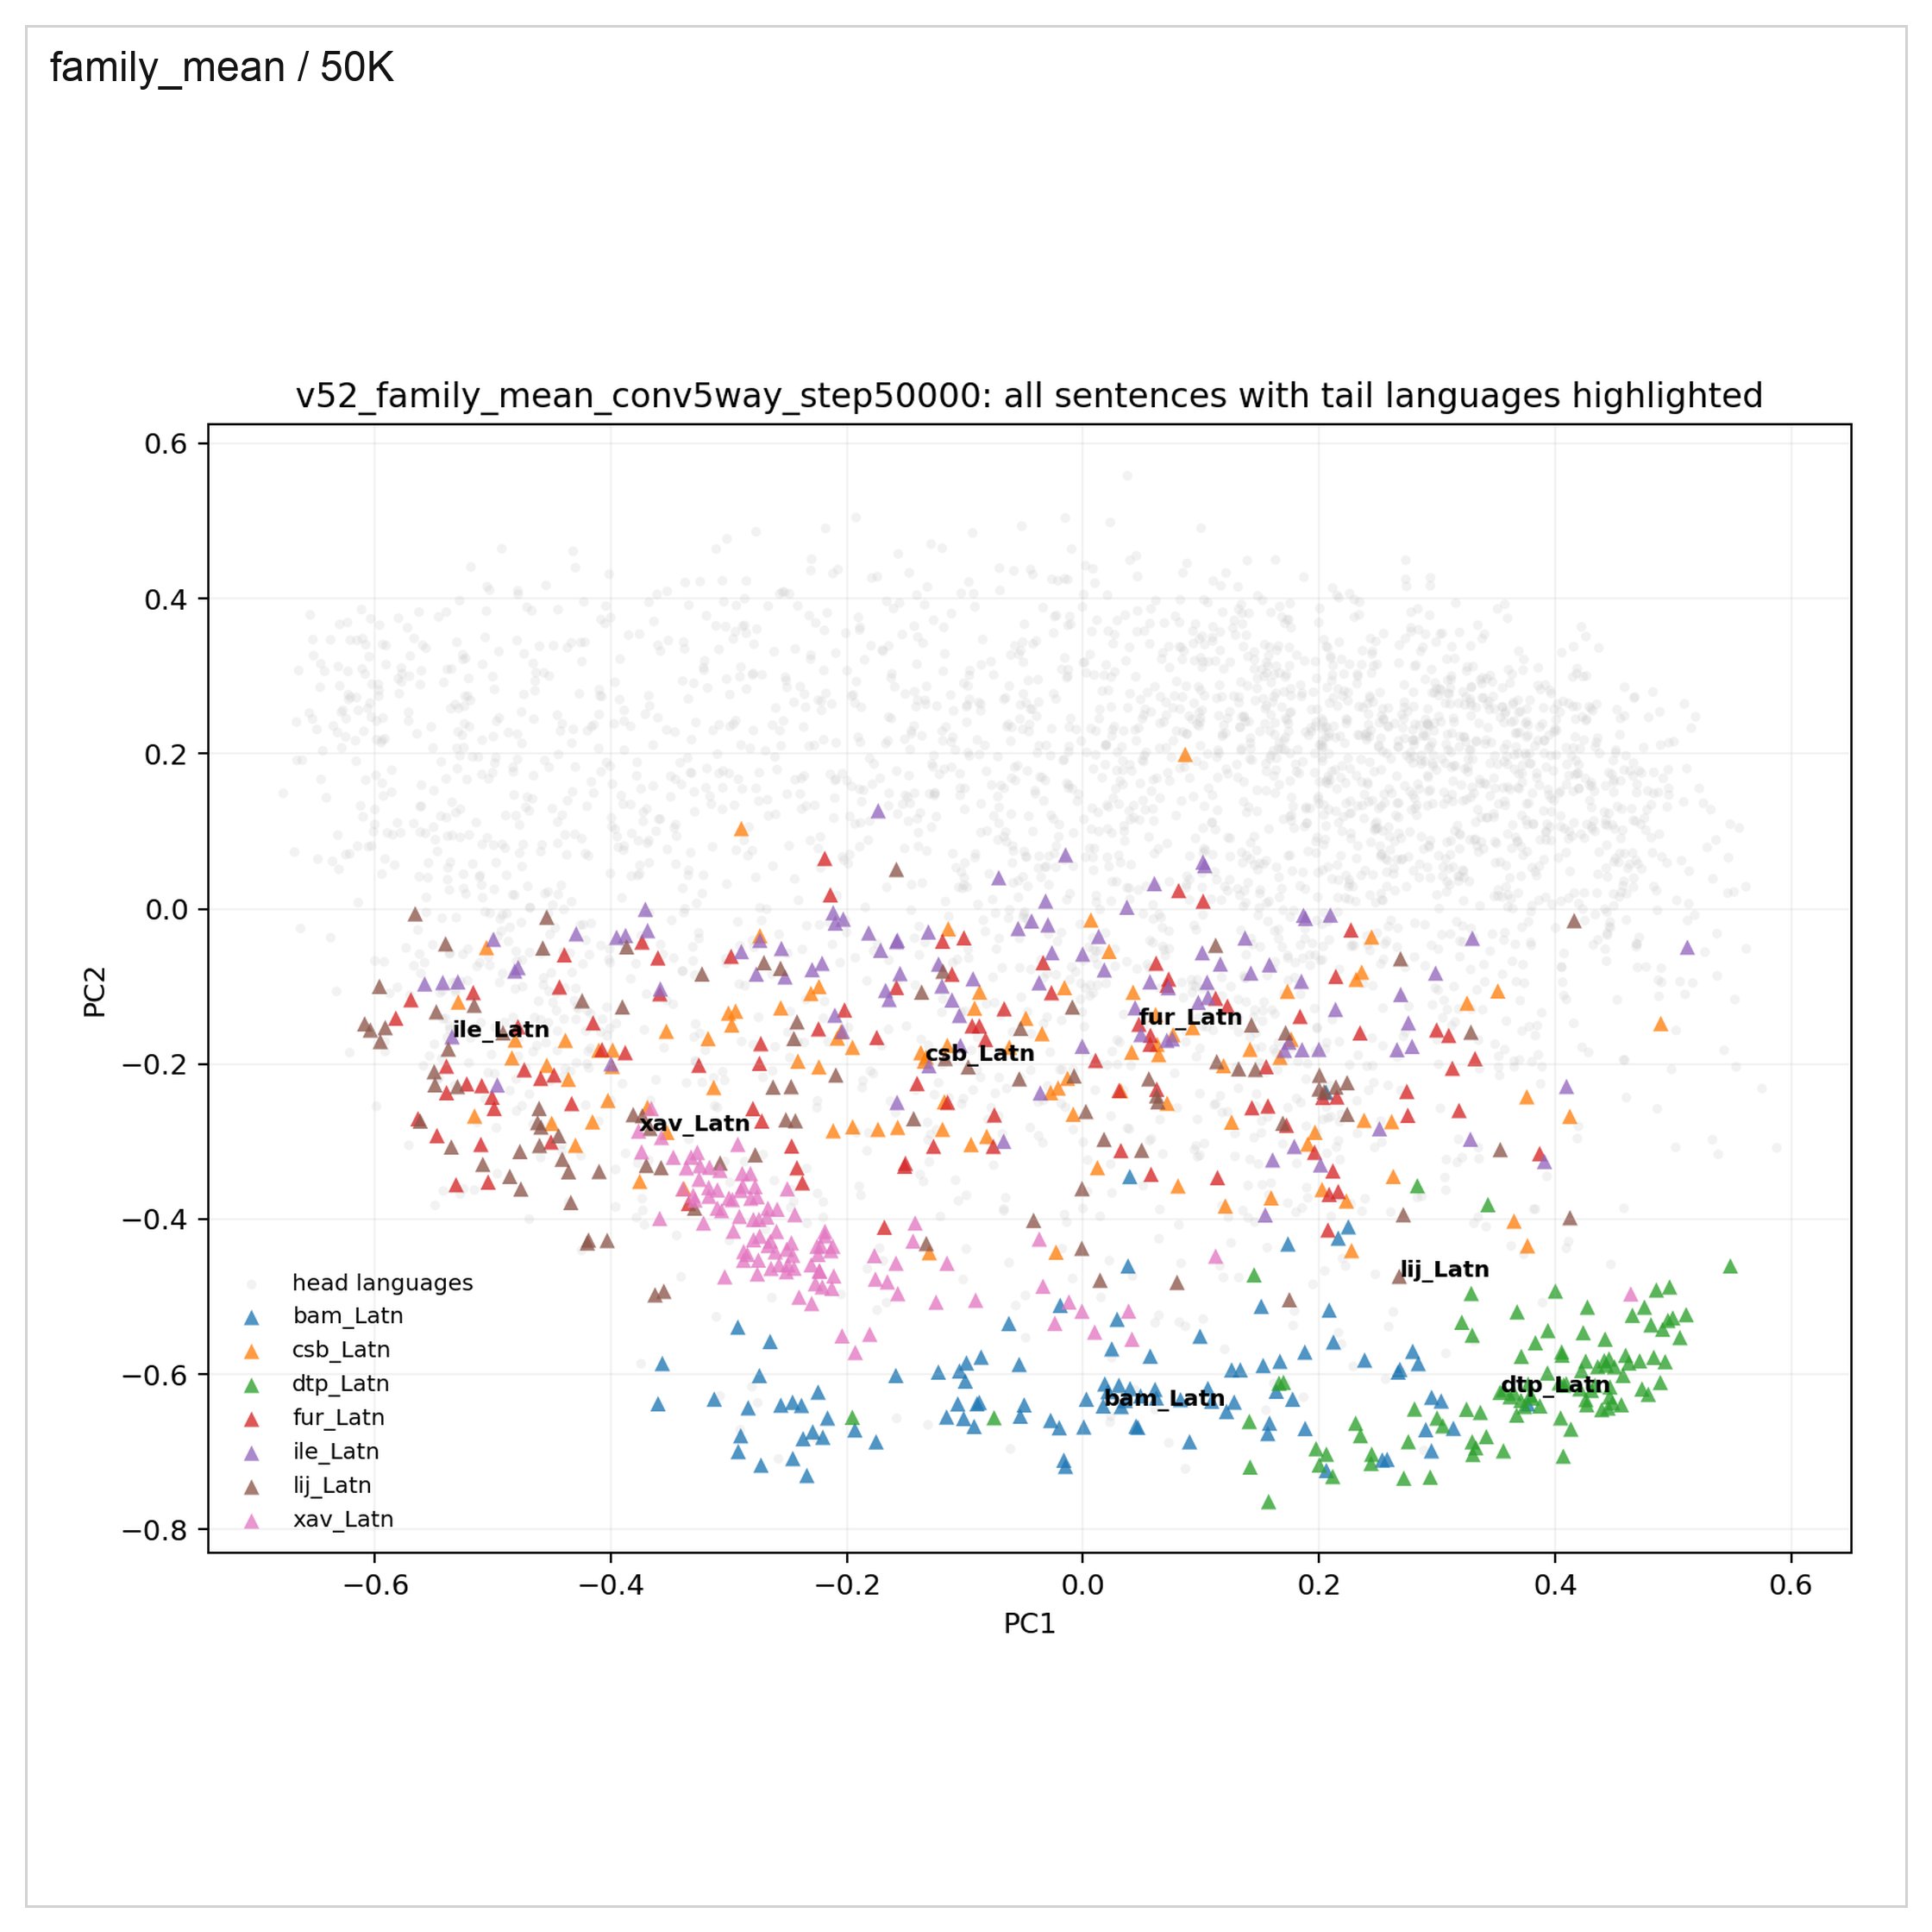
\includegraphics[width=\linewidth]{mapgrid_07.png}
\caption{초기화 방법별·step별 2D embedding map 전체(7/7): \famm\ 50K.}
\end{figure}

\clearpage
\subsection{38개 언어 centroid 2D map}
그림~\ref{fig:centroidmap}은 \fvt\ 50K checkpoint에서 sampled 38개 언어의 sentence-vector centroid를 2D PCA로 나타낸 것이다. 삼각형은 Target7 tail 언어이고, 원은 head/reference 언어이다.

\begin{figure}[H]\centering
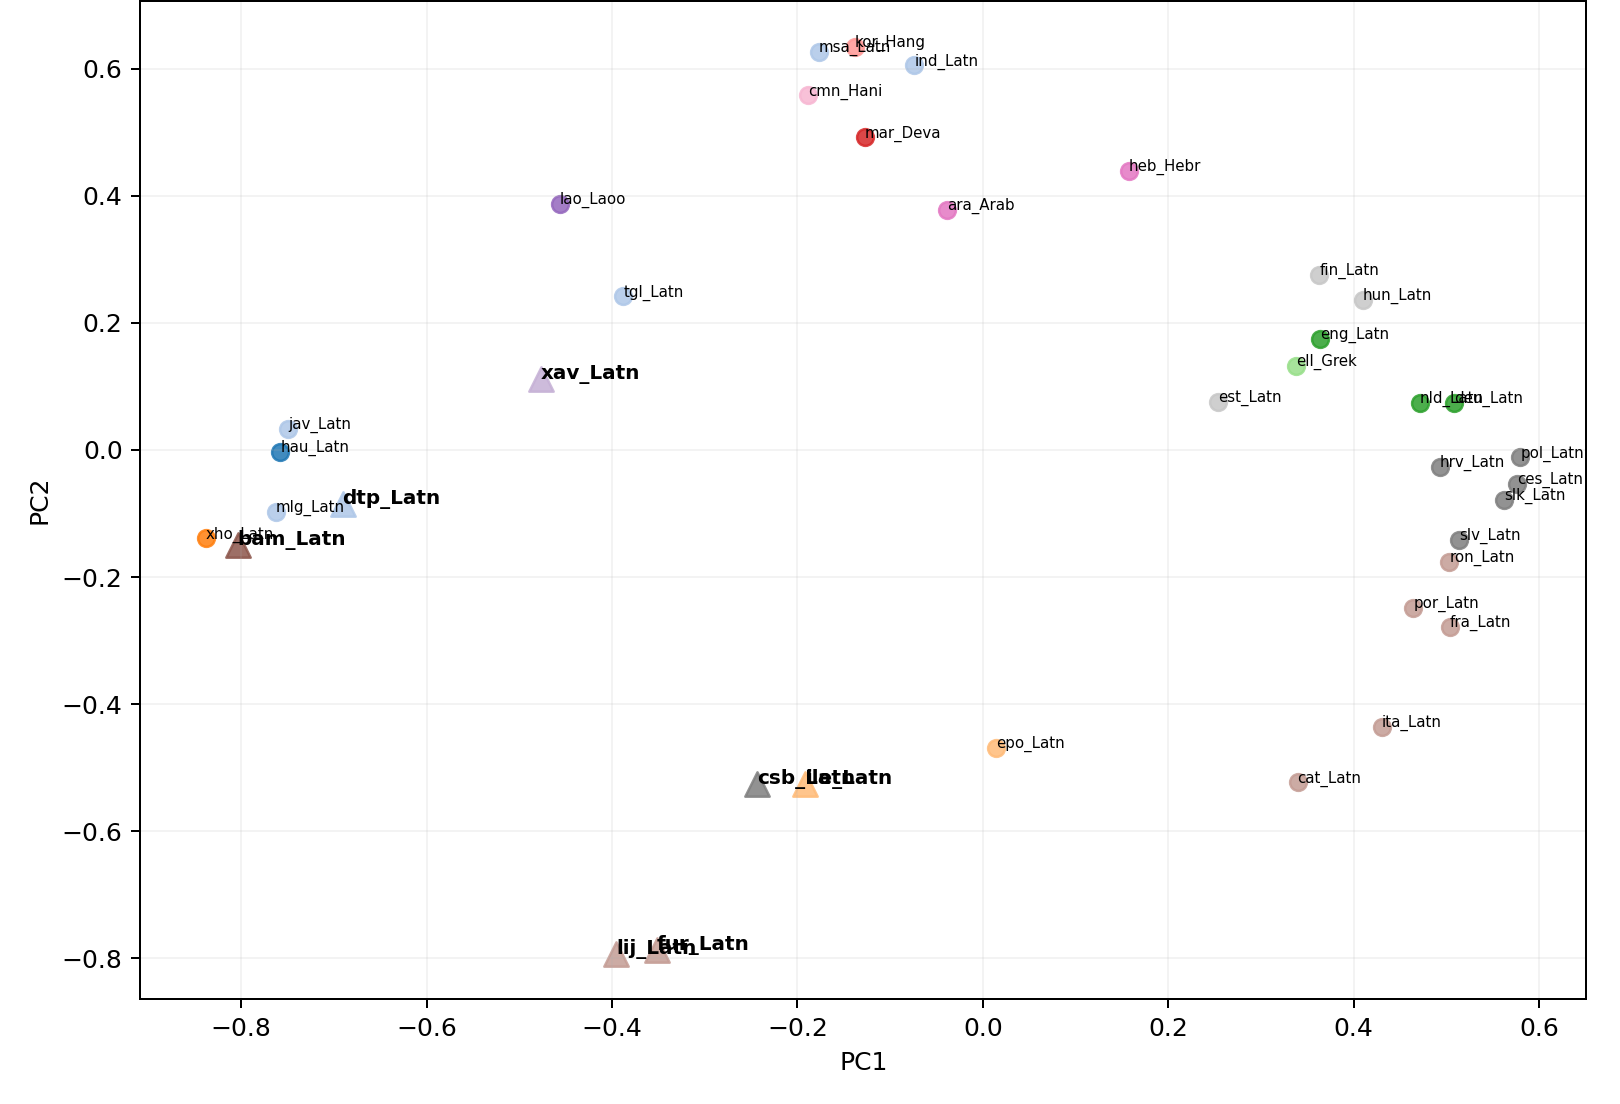
\includegraphics[width=0.88\linewidth]{centroid_fvt_50k.png}
\caption{38개 언어 centroid의 2D PCA map(\fvt, 50K). Target7은 삼각형으로 표시하고, 나머지 head/reference 언어는 원으로 표시한다.}
\label{fig:centroidmap}
\end{figure}

\end{document}
